\documentclass[11pt]{article}
\usepackage[T1]{fontenc}
\usepackage{lmodern}
\usepackage[margin=1in]{geometry}
\usepackage{amsmath,amssymb,amsthm,mathtools}
\usepackage{microtype}
\usepackage[numbers,sort&compress]{natbib}
\usepackage{xcolor}
\usepackage{tikz}
\usetikzlibrary{arrows.meta,positioning,calc}
\usepackage[colorlinks=true,linkcolor=blue!45!black,citecolor=blue!45!black,urlcolor=blue!45!black]{hyperref}
\hypersetup{pdftitle={The abelian Zilber--Pink conjecture},pdfauthor={OpenAI}}
\pdfinfoomitdate=1
\pdftrailerid{}
\pdfsuppressptexinfo=15
\newtheorem{theorem}{Theorem}[section]
\newtheorem{lemma}[theorem]{Lemma}
\newtheorem{proposition}[theorem]{Proposition}
\newtheorem{corollary}[theorem]{Corollary}
\theoremstyle{definition}
\newtheorem{definition}[theorem]{Definition}
\theoremstyle{remark}
\newtheorem{remark}[theorem]{Remark}
\numberwithin{equation}{section}
\newcommand{\Qbar}{\overline{\mathbb Q}}
\newcommand{\cA}{\mathcal A}
\DeclareMathOperator{\Lie}{Lie}
\DeclareMathOperator{\Hom}{Hom}
\DeclareMathOperator{\End}{End}
\DeclareMathOperator{\codim}{codim}
\DeclareMathOperator{\rank}{rank}
\DeclareMathOperator{\Atyp}{Atyp}
\setlength{\emergencystretch}{1em}
\raggedbottom

\title{The abelian Zilber--Pink conjecture}
\author{OpenAI}
\date{September 24, 2026}
\begin{document}
\maketitle
\begin{abstract}
We prove the abelian Zilber--Pink conjecture over
$\overline{\mathbb Q}$. Every irreducible subvariety of an abelian variety
has only finitely many maximal atypical subvarieties, where atypicality
is measured inside its smallest containing torsion coset.
\end{abstract}
\begingroup
\setcounter{tocdepth}{1}
\tableofcontents
\endgroup
\clearpage
\section{Introduction}\label{sec:introduction}

A dimension count predicts how a subvariety of an abelian variety
meets a fixed torsion coset. The abelian Zilber--Pink conjecture asks
for a finiteness statement when the intersection is larger than this
prediction, even though the torsion coset is allowed to vary. We prove
the conjecture over number fields in arbitrary dimension.

\subsection{The finiteness statement}
Fix a number field $K$, an algebraic closure $\bar K$, and an abelian
variety $A/K$. All subvarieties below are closed and irreducible over
$\bar K$. A \emph{special subvariety} of $A_{\bar K}$ is a torsion coset
$B+\tau$, where $B$ is an abelian subvariety and $\tau$ is a torsion
point. For a subvariety $Z$, write $\langle Z\rangle_{\mathrm{sp}}$ for
the smallest special subvariety containing $Z$.

This smallest subvariety exists: choose a special subvariety of least
dimension containing $Z$, and intersect it with any other such
subvariety. Each irreducible component of a nonempty intersection of
torsion cosets is a torsion coset. The component containing $Z$ has the
same dimension as the chosen one, and hence equals it. This also proves
uniqueness and the implication
\begin{equation}\label{eq:closure-monotonicity}
 Z\subseteq Z'\quad\Longrightarrow\quad
 \langle Z\rangle_{\mathrm{sp}}\subseteq
 \langle Z'\rangle_{\mathrm{sp}}.
\end{equation}
Here the assertion about intersections follows by intersecting the
underlying algebraic subgroups: a nonempty intersection is a coset of
their intersection, torsion points lift through surjective homomorphisms of abelian
varieties, and every component of an algebraic subgroup of an abelian
variety contains a torsion point.

Let $X\subseteq A_{\bar K}$ and put $S=\langle X\rangle_{\mathrm{sp}}$.
An irreducible component $Y$ of $X\cap T$, for a special $T\subseteq S$,
is \emph{atypical for $X$ in $S$} if
\begin{equation}\label{eq:atypical}
 \dim Y>\dim X+\dim T-\dim S.
\end{equation}
Maximality of an atypical subvariety always means maximality for
inclusion among the atypical subvarieties of $X$ in $S$.

\begin{theorem}\label{thm:main}
For every number field $K$, every abelian variety $A/K$, and every
irreducible subvariety $X\subseteq A_{\bar K}$, there are only finitely
many maximal atypical subvarieties of $X$ in
$S=\langle X\rangle_{\mathrm{sp}}$. Equivalently, there are finitely many
proper atypical subvarieties $Y_1,\ldots,Y_m\subsetneq X$ such that every
atypical subvariety is contained in one of the $Y_j$.
\end{theorem}

The list can be empty. No bound on the degrees or heights of the
intersection points is assumed, and no simplicity, endomorphism, or
complex multiplication hypothesis is imposed on $A$.
The theorem concerns torsion cosets in abelian varieties; it gives no
effective or uniform bound for the number of maximal atypical
subvarieties.

For a torsion coset $S$ and an integer $r\ge0$, set
\[
 S^{[r]}=\bigcup_{\substack{T\subseteq S\ \mathrm{special}\\
                         \codim_S T\ge r}}T.
\]
We first prove the following non-density theorem, with universal
quantifiers on the ambient abelian variety and its subvarieties.

\begin{theorem}\label{thm:nondensity}
Let $A$ be an abelian variety over $\Qbar$, and let $X\subseteq A$ be an
irreducible subvariety contained in no proper torsion coset. Then
$X\cap A^{[\dim X+1]}$ is not Zariski dense in $X$.
\end{theorem}

The passage from this assertion to Theorem~\ref{thm:main} uses the
optimal-subvariety reduction of Barroero and Dill. Section~\ref{sec:finiteness}
checks its universal hypotheses and gives the final inclusion argument.
In particular, the proof does not stop with non-density for one fixed
$X$.

The same universal non-density theorem also gives a consequence for
translations by finite-rank subgroups. For point sets
$E,\Gamma\subseteq A(\Qbar)$, write
$E+\Gamma=\{e+\gamma:e\in E,\ \gamma\in\Gamma\}$.

\begin{corollary}[Finite-rank translated intersections]
\label{cor:finite-rank-translates}
Let $A$ be an abelian variety over $\Qbar$, let
$\Gamma\subseteq A(\Qbar)$ be a subgroup satisfying
\[
 \dim_{\mathbb Q}\bigl(\Gamma\otimes_{\mathbb Z}\mathbb Q\bigr)<\infty,
\]
and let $X\subseteq A$ be an irreducible closed subvariety of dimension
$d$ contained in no translate of a proper algebraic subgroup of $A$.
Then
\[
 X(\Qbar)\cap\bigl(A^{[d+1]}(\Qbar)+\Gamma\bigr)
\]
is not Zariski dense in $X$. If $d=1$, this intersection is finite.
\end{corollary}

This is the abelian algebraic-point case of Pink's
Conjecture~5.2 \cite{Pink2005}. The group $\Gamma$ need not be finitely
generated: torsion subgroups and division hulls of finitely generated
subgroups are included. Section~\ref{sec:finite-rank} applies Pink's
reduction \cite[Theorem~5.3]{Pink2005} and records where the stronger
no-proper-translate hypothesis is used.

\subsection{Historical context}
Zilber formulated the unlikely-intersection principle for semiabelian
varieties \cite{Zilber2002}. Pink's semiabelian formulation
\cite[Conjecture~5.1]{Pink2005} specializes to the high-codimension
non-density statement considered here.

The torsion-point case belongs to the Manin--Mumford theorem of Raynaud
\cite[p.~327, Th\'eor\`eme]{Raynaud1983Torsion}: a subvariety with dense
torsion points is a torsion coset. Unlikely intersections allow the torsion points to be
replaced by torsion cosets of varying positive dimensions. Even when
these cosets have large codimension, their intersections can contain
positive-dimensional components; the maximality condition in
Theorem~\ref{thm:main} accounts for this possibility.

For curves in powers of a CM elliptic curve, Viada proved
codimension-two finiteness under the hypothesis that the curve lies in
no translate of a proper algebraic subgroup
\cite[Theorem~2]{Viada2003}. R\'emond and Viada removed this
transversality restriction, retaining the necessary exclusion of proper
algebraic subgroups \cite[Theorem~1.7]{RemondViada2003}. Habegger and Pila proved
finiteness for curves in arbitrary abelian varieties over number fields
\cite[Theorem~1.1]{HabeggerPila2016}. Barroero, K\"uhne and Schmidt
subsequently established the corresponding curve theorem for general
semiabelian varieties over number fields
\cite[Theorem~1.1]{BarroeroKuhneSchmidt2023}.
More recently, Dogra and Pandit obtained bounded-degree results for smooth
curves whose Jacobians surject onto the ambient abelian variety. Together
with established height bounds, these give finiteness. Their local theorem
gives explicit reduction bounds under good-reduction and genus hypotheses,
and cardinality bounds under further restrictions on the simple isogeny factors
\cite[Theorem~1 and Corollary~1]{DograPandit2026}.

Higher-dimensional non-density was known under additional geometric
or height restrictions. For positive-dimensional $X$, consider the
condition
\[
 \dim\pi(X)=\min\{\dim X,\dim(A/B)\}
 \qquad\text{for every quotient }\pi:A\longrightarrow A/B.
\]
In the CM case, R\'emond proved finite-rank translated non-density under
this condition \cite[Theorem~1.3]{Remond2009}; Habegger independently
proved the untranslated case \cite[Corollary~2]{Habegger2009}.
Viada obtained a non-CM elliptic-power case
\cite[Theorem~1.3]{Viada2009}. Habegger and Pila established
non-density under the same quotient condition for arbitrary abelian
varieties \cite[Theorem~1.3(ii)]{HabeggerPila2016}. Without that condition,
their Theorem~1.3(i) gives non-density at every fixed height bound when
$X$ is contained in no proper torsion coset.

There were also higher-dimensional finiteness results for maximal
atypical subvarieties. Habegger and Pila's results imply finiteness of
those of codimension one in $X$
\cite[Theorem~9.14(i)]{HabeggerPila2016}. For codimension-two
subvarieties of powers of an elliptic curve contained in no proper
torsion coset, maximal-atypical finiteness was proved in the CM case by
Checcoli, Veneziano and Viada \cite[Corollary~1.5]{CheccoliVenezianoViada2014}
and without the CM restriction by Hubschmid and Viada
\cite[Theorem~1.1]{HubschmidViada2019}.
Theorem~\ref{thm:main} treats arbitrary abelian varieties and all
codimensions, without the additional quotient-dimension or height
restrictions.

The geometric inputs are Ax's analytic-subgroup theorem
\cite{Ax1972}, in the precise analytic-subset form stated in
\cite[Theorem~5.3]{HabeggerPila2016}, and the finiteness of directions of
geodesic-optimal subvarieties of a fixed parent
\cite[Proposition~6.1]{HabeggerPila2016}.
Habegger and Pila explicitly attribute the latter finiteness to earlier
results of R\'emond \cite[Lemma~2.6 and Proposition~3.2]{Remond2009}.

The height argument follows Vojta's curve method \cite{Vojta1991},
Faltings' extension to abelian varieties \cite{Faltings1991}, and
R\'emond's generalized inequality \cite{Remond2005Vojta}. We use Dill's
version with separate height thresholds for the factors; his introduction
credits Ange with the preceding extension to different projective
varieties \cite{Dill2020}.
The bounded-scale argument adapts the two-measure comparison in the
Bogomolov proofs of Ullmo and Zhang \cite{Ullmo1998,Zhang1998}, based
on Szpiro--Ullmo--Zhang equidistribution \cite{SzpiroUllmoZhang1997}.
Zhang's account \cite[Section~3]{Zhang1998ICM} explicitly traces the
consecutive-difference map to Faltings. The metric-variation calculation
uses Yuan's arithmetic bigness method \cite{Yuan2008}, in the nef adelic
form of Yuan and Zhang \cite{YuanZhang2021}. The local weighted-index
argument follows Faltings' method, and the final cut uses his product
theorem in Evertse's explicit form \cite{Evertse1995Product}.

The estimates proved here keep these inputs uniform across
several height scales and across auxiliary varieties with bounded
fields of definition. The argument for the bounded scale compares
measures only on the fixed low factor; it does not invoke an
equidistribution theorem for a fixed variety as a substitute for
uniformity.

\subsection{Proof strategy and organization}

The proof studies a hypothetical Zariski-generic sequence of
high-codimension intersection points. The square roots of their
N\'eron--Tate heights need not be comparable. Repeatedly taking a quotient
of largest dimension on which the height is smaller separates the ambient variety,
up to isogeny, into at most one bounded level and finitely many successively
larger unbounded levels. Normalizing each level separately makes the
point vectors bounded. Their algebraic subgroup relations then converge
to a real-endomorphism projector that sends the normalized vectors to
zero in the limit.

The auxiliary sequence theorem in Section~\ref{sec:sequences} excludes
the high-codimension limit just obtained. Its geometric input is uniform tangent
positivity, obtained in Section~\ref{sec:tangent} from Ax's theorem and
the finiteness of geodesic-optimal directions in a fixed parent variety.
Projection to smaller abelian varieties handles every possible failure
of this positivity.

There are two arithmetic parts. When every height level is unbounded,
Section~\ref{sec:high} applies Dill's generalized Vojta--R\'emond
inequality. The relevant multiplicative constant is independent of the
accuracy of a rational approximation to the limiting projector.
This permits the approximation error to be made small before taking
points of sufficiently large height.

A bounded level requires a different argument. Section~\ref{sec:minimal}
chooses auxiliary products of minimal dimension whose degrees and fields
of definition are bounded. These bounds concern the varieties, while
the marked points may have arbitrarily large degree. A zero-dimensional
bounded factor reduces to the unbounded case. For a positive-dimensional
bounded factor, Section~\ref{sec:arithmetic} proves a uniform arithmetic
intersection lower bound. The proof compares two limiting measures on
that fixed factor: one from a product map and one from a consecutive
difference map. The first has positive density at a suitable diagonal
point; the second has zero density there. A variational argument on the
changing varieties converts this disagreement into arithmetic positivity.

Small sections supplied by that positivity have a uniformly positive
weighted vanishing index at the marked points
(Section~\ref{sec:index}). The product theorem then yields a proper
factor through a marked point. A multiplicity calculation bounds both
its degree and the number of its Galois conjugates
(Section~\ref{sec:product-cut}). This contradicts minimality and completes the sequence theorem.

\subsection{Conventions}
We identify $\bar K$ with $\Qbar$ and fix an embedding $\Qbar\hookrightarrow
\mathbb C$. A coset without the adjective special may be translated by
an arbitrary point. Its direction is the abelian subvariety being
translated. All logarithmic heights and arithmetic intersection numbers
are absolute, normalized by the degree of the field of definition.
Constants in asymptotic estimates may depend on fixed varieties,
embeddings and polarizations, but not on the sequence index unless
explicitly stated. The notation $u_i\asymp v_i$ means that both ratios
are bounded above by positive constants.

\section{Height scales and an auxiliary sequence theorem}
\label{sec:sequences}

The proof separates coordinates whose heights grow at different rates.
We first explain the linear algebra that permits real homomorphisms to act
on normalized points. We then state the sequence theorem and show that it
implies Theorem~\ref{thm:nondensity}. Its proof occupies the subsequent
sections.

\subsection{Real homomorphisms and height norms}

For an abelian variety $G$ over $\Qbar$, choose a symmetric ample line
bundle and write
\[
 \mathcal H(G)=G(\Qbar)\otimes_{\mathbb Z}\mathbb R,
 \qquad \|x\|^2=\widehat h(x).
\]
The canonical height pairing extends to a positive-definite real
quadratic form on $\mathcal H(G)$. Indeed, every finite collection of
points is defined over one number field, and the assertion on its real
span is the positive definiteness of the N\'eron--Tate pairing on the
Mordell--Weil group modulo torsion. We use the same notation for a point
and its image in $\mathcal H(G)$. In particular, torsion points have image
zero. Polarizations also give Hermitian forms on the complex Lie algebras
$\Lie(G)$. On products we choose product polarizations and product norms.
We use the standard complex uniformization, complete reducibility,
finite-rank homomorphism groups and polarization adjoints recalled in
\cite[Chapter~I, Sections~2, 10 and 14]{Milne2008AV}. Canonical metrics
and heights are taken with the multiplication normalization of
\cite[Theorem~2.2]{Zhang1995}.

\begin{lemma}[Real homomorphism calculus]
\label{lemma:real-calculus}
Let $G,G'$ be abelian varieties over $\Qbar$ with the preceding choices.
Every element of
$\Hom(G,G')_{\mathbb R}=\Hom(G,G')\otimes_{\mathbb Z}\mathbb R$
acts on both $\Lie(G)$ and $\mathcal H(G)$. The Lie action is faithful.
Convergence in this finite-dimensional real homomorphism space implies
operator-norm convergence on the height spaces.

The polarization adjoint of a real homomorphism is a real homomorphism.
Its kernel and image in the Lie algebras have orthogonal projectors in
the corresponding real endomorphism algebras, and it has a generalized
inverse in the opposite real homomorphism space. In particular, if $f$
is fixed and $\|f(x_i)\|\to0$, then
\[
 \|P_{(\ker f)^\perp}(x_i)\|\longrightarrow0.
\]
\end{lemma}

\begin{proof}
Fix integral homomorphisms $f_1,\ldots,f_b$ forming a real basis of
$\Hom(G,G')_{\mathbb R}$. For each $j$, ample domination of $f_j^*L'$
by a power of $L$ gives
$\widehat h_{L'}(f_j(x))\le C_j\widehat h_L(x)$ for all algebraic
points $x$. The same inequality holds on $\mathcal H(G)$, by its
quadratic-form interpretation on every finite-dimensional span. Hence
\[
 \left\|\sum_j t_j f_j(x)\right\|
 \le \left(\sum_j |t_j|\sqrt{C_j}\right)\|x\|.
\]
The constants are independent of the fields of definition of the
points. This proves the assertion about operator norms.

The underlying real Lie representation identifies with the real
extension of the representation on rational homology. It is faithful,
also after scalar extension from $\mathbb Q$ to $\mathbb R$. The
polarization adjoint belongs to rational homomorphisms, and therefore
extends to real homomorphisms. For a real homomorphism $f$, the operator
$f^*f$ is nonnegative and self-adjoint on $\Lie(G)$. Choose a real
polynomial $p$ that is zero at zero and equals $1/t$ at every positive
eigenvalue $t$ of $f^*f$. Then
\[
 f^\dagger=p(f^*f)f^*
\]
is a real homomorphism and
$f^\dagger f=P_{(\ker f)^\perp}$,
$ff^\dagger=P_{\operatorname{im}f}$.
Faithfulness makes these identities identities of real homomorphisms,
so they also hold on the height spaces. The last assertion follows by
applying the fixed bounded operator $f^\dagger$.
\end{proof}

In particular, the image of any real homomorphism into $G$ is the image
of a real idempotent endomorphism of $G$. Images, inverse images, and
intersections of finitely many such Lie subspaces can therefore be
handled by real homomorphisms. These subspaces need not be Lie algebras
of abelian subvarieties.

\subsection{The sequence theorem}

Local fiber dimension at a point always means the maximum of the
dimensions of the irreducible components of the fiber through that
point. This convention matters when a marked point is singular.

The fiber bounds in the sequence theorem record the dimension
contributed by each height level. Let $W_1,W_2$ be abelian varieties.
Consider an irreducible $X\subseteq W_1\times W_2$, points
$(p_{i1},p_{i2})\in X$, and scales $H_{i\ell}\ge1$ with
$\|p_{i\ell}\|=O(\sqrt{H_{i\ell}})$ and
$H_{i1}/H_{i2}\to0$. Retain the first coordinate when forming the
second ambient factor:
\[
 \begin{array}{lll}
 A_1=W_1,&Y_1=\operatorname{pr}_1(X),&m_1=\dim Y_1,\\
 A_2=W_1\times W_2,&Y_2=X,&m_2=\dim X-\dim Y_1.
 \end{array}
\]
The distinguished subgroups are $W_1\subseteq A_1$ and
$\{0\}\times W_2\subseteq A_2$. The integers $m_1,m_2$ are the
generic dimensions of the corresponding fibers, and
$m_1+m_2=\dim X$. The copied coordinate
$p_{i1}/\sqrt{H_{i2}}$ tends to zero, so it disappears after
normalization at the second scale. In the reduction below, genericity
of the sequence ensures that the marked points eventually have these
fiber dimensions. The following definition allows arbitrary pairs
$W_\ell\subseteq A_\ell$, accommodating both this construction with
any number of levels and the quotients used in Section~\ref{sec:tangent}.

\begin{definition}[Sequence data]
\label{def:sequence-data}
Let $I$ be the ordered list $1,\ldots,s$, possibly preceded by $0$.
The list is nonempty; if $0$ occurs, $s$ may be zero. For each
$\ell\in I$, fix an abelian variety $A_\ell$ over $\Qbar$, a nonzero
abelian subvariety $W_\ell\subseteq A_\ell$, an irreducible subvariety
$Y_\ell\subseteq A_\ell$, and an integer $m_\ell\ge0$. Put
\[
 \cA=\prod_{\ell\in I}A_\ell,
 \qquad W=\prod_{\ell\in I}W_\ell,
 \qquad D_\ell=A_\ell/W_\ell.
\]
For positive integers $i$, let $y_{i\ell}\in Y_\ell(\Qbar)$ and
$H_{i\ell}\ge1$ satisfy
\begin{equation}
 \label{eq:sequence-fibers}
 \dim_{y_{i\ell}}\bigl(Y_\ell\cap(y_{i\ell}+W_\ell)\bigr)
 \le m_\ell,
 \qquad \|y_{i\ell}\|=O(\sqrt{H_{i\ell}}).
\end{equation}
For consecutive indices $\ell,\ell'$ in $I$, require
$H_{i\ell}/H_{i\ell'}\to0$.

The factors $\ell\ge1$ are called high factors. They satisfy
$H_{i\ell}\to\infty$, and, for every fixed homomorphism
$g:A_\ell\to G$ to an abelian variety whose restriction to $W_\ell$
is nonzero,
\begin{equation}
 \label{eq:sequence-nondegenerate}
 \liminf_{i\to\infty}
 \frac{\|g(y_{i\ell})\|}{\sqrt{H_{i\ell}}}>0.
\end{equation}
If the index $0$ occurs, it is called the low factor and satisfies
$W_0=A_0$, $H_{i0}=1$. Its points eventually avoid each fixed proper
torsion coset of $A_0$.
\end{definition}

The homomorphism in \eqref{eq:sequence-nondegenerate} is integral; the
condition is equivalently unchanged by allowing rational homomorphisms.
Its positive lower bound may depend on $g$. No bound on the degrees of
the marked points is assumed.

\begin{theorem}[Auxiliary sequence theorem]
\label{thm:sequence}
For sequence data as in Definition~\ref{def:sequence-data}, let
$V\subseteq\Lie(W)$ be the image of an idempotent in
$\End(\cA)_{\mathbb R}$. Let $\Phi$ be the orthogonal projector with
kernel $V$, and put
\[
 q_i=(y_{i\ell}/\sqrt{H_{i\ell}})_{\ell\in I}
 \in\mathcal H(\cA).
\]
The following two conditions cannot both hold:
\begin{equation}
 \label{eq:forbidden-sequence}
 \codim_{\Lie(W)}V>\sum_{\ell\in I}m_\ell,
 \qquad \|\Phi(q_i)\|\longrightarrow0.
\end{equation}
\end{theorem}

We will first prove this theorem for all-high data in every dimension.
We then treat data with a low factor. At each stage, a hypothetical
counterexample of least $\dim\cA$ gives the geometric exclusion proved
in Section~\ref{sec:tangent}. The order of these two stages permits a
projection that removes the low factor.

\subsection{Decomposing a sequence into height scales}

\begin{lemma}[Height decomposition]
\label{lemma:height-decomposition}
Let $A$ be a nonzero abelian variety and $x_i\in A(\Qbar)$. After
passing to a subsequence, there is an isogeny
\[
 \alpha:A\longrightarrow\prod_{\ell\in I}W_\ell
\]
with nonzero factors, and scales $H_{i\ell}\ge1$, such that the
coordinates $p_{i\ell}$ of $\alpha(x_i)$ have norms
$O(\sqrt{H_{i\ell}})$ and successive scale ratios tend to zero.
There is at most one bounded scale, placed first and equal to one.
Every other scale tends to infinity and satisfies
\eqref{eq:sequence-nondegenerate} with $A_\ell=W_\ell$ for every
fixed nonzero homomorphism on $W_\ell$.
\end{lemma}

\begin{proof}
If the point heights are bounded, use $A$ itself as the bounded factor.
Otherwise take a subsequence with $H_i=\|x_i\|^2\to\infty$.
Among fixed quotient homomorphisms $\pi:A\to Q$ for which
$\|\pi(x_i)\|^2=o(H_i)$ on some subsequence, choose one with
maximal $\dim Q$, and restrict to that subsequence. The zero quotient
is allowed. A quotient of dimension $\dim A$ is an isogeny and cannot
have this property, by height comparison. Poincar\'e reducibility
provides an isogeny $A\to Q\times W'$ whose first component is
$\pi$; harmless fixed isogenies of the targets can be absorbed here.

Write $p'_i$ for the $W'$ coordinate. Suppose a fixed nonzero
homomorphism $g$ on $W'$ satisfies
\[
 \liminf_{i\to\infty}\frac{\|g(p'_i)\|}{\sqrt{H_i}}=0.
\]
Take a further subsequence on which this ratio tends to zero. The homomorphism
whose coordinates are $\pi$ and $g$ on the complementary factor has
image of dimension $\dim Q+\dim g(W')>\dim Q$, and its point
heights are $o(H_i)$. Quotienting by the identity component of its
kernel changes its image only by an isogeny. This contradicts the
maximality of $Q$. Thus $W'$ is a high factor with scale $H_i$ and the
required nondegeneracy for every fixed homomorphism.

If $Q=0$, stop. Otherwise continue on $Q$ with the points
$\pi(x_i)$. If their heights are
bounded, this is the low factor; if not, extract a diverging scale and
repeat. At each step the remaining quotient has smaller dimension and
its squared heights are little-oh of the preceding scale. The process
therefore terminates. Reverse the order of the extracted factors, so
that the scales are increasing. Composing the finitely many fixed
isogenies gives $\alpha$. Fixed height comparisons preserve all the
asserted bounds and ratios.
\end{proof}

\begin{proposition}
\label{prop:sequence-implies-nondensity}
The auxiliary sequence theorem implies Theorem~\ref{thm:nondensity}
for every abelian variety over $\Qbar$.
\end{proposition}

\begin{proof}
Let $X\subseteq A$ be irreducible and contained in no proper torsion
coset. If $\dim A=0$, there are no torsion cosets of codimension
$\dim X+1$, so there is nothing to prove. Suppose otherwise that
$X\cap A^{[\dim X+1]}$ is Zariski dense. Since $\Qbar$ is
countable, choose a sequence in this intersection that eventually
avoids every fixed proper closed subset of $X$ defined over $\Qbar$.
Apply Lemma~\ref{lemma:height-decomposition} and replace $A,X$ and
the sequence by their isogeny images. Dimensions of subvarieties and
codimensions of torsion cosets are preserved by this finite map. Its
image $X$ is still contained in no proper torsion coset. We have now
written $A=\prod_{\ell\in I}W_\ell$ and
$x_i=(p_{i\ell})_\ell$.

For each $i$, choose a torsion coset $B_i+\tau_i$ containing $x_i$
with $\codim_A B_i>\dim X$. After extraction its codimension is
constant. In $\Lie(A)$ let
\[
 U_i=\operatorname{diag}(H_{i\ell}^{-1/2})\Lie(B_i).
\]
The orthogonal projector $P_i$ onto $U_i$ is a real endomorphism by
Lemma~\ref{lemma:real-calculus}, applied to the scaled subgroup
inclusion. All these projectors have the same rank. A subsequence
converges to an orthogonal projector $P$ of the same rank. Moreover
$P\in\End(A)_{\mathbb R}$, because this finite-dimensional
subspace is closed in the space of real linear maps on $\Lie(A)$.
Put $U=\operatorname{im}P$. Then
\begin{equation}
 \label{eq:initial-limit-projector}
 \codim_{\Lie(A)}U>\dim X,
 \qquad
 \left\|(1-P)(p_{i\ell}/\sqrt{H_{i\ell}})_\ell\right\|
 \longrightarrow0.
\end{equation}
For the second assertion, torsion vanishes in the height space, so
$1-P_i$ kills the indicated normalized vector exactly. Those vectors
are bounded, and Lemma~\ref{lemma:real-calculus} converts convergence
of the projectors into degree-independent operator-norm convergence.

To obtain the local fiber bounds in the sequence theorem, we retain
copies of all slower coordinates. For each $\ell\in I$ set
\[
 A_\ell=\prod_{h\le\ell}W_h,
 \qquad Y_\ell=\operatorname{pr}_{\le\ell}(X),
 \qquad y_{i\ell}=(p_{ih})_{h\le\ell}.
\]
Regard $W_\ell$ as the last coordinate in $A_\ell$. Let
$m_\ell=\dim Y_\ell-\dim Y_{\ell^-}$, where $Y_{\ell^-}$ is
the preceding projection and is a point for the first index. These
integers are nonnegative and sum to $\dim X$. The local dimension of
the fiber of $Y_\ell\to Y_{\ell^-}$ equals $m_\ell$ on a
nonempty open subset. The sequence eventually lies in that subset:
the inverse image in $X$ of its complement is a fixed proper closed
set. Thus \eqref{eq:sequence-fibers} holds after discarding finitely
many terms.

For a high factor, every slower coordinate is
$o(\sqrt{H_{i\ell}})$ in norm. A fixed homomorphism on $A_\ell$
nonzero on its last $W_\ell$ coordinate is the sum of a nonzero
homomorphism on that coordinate and fixed homomorphisms on the slower
ones. The triangle inequality and
Lemma~\ref{lemma:height-decomposition} prove
\eqref{eq:sequence-nondegenerate}. If a low factor occurs, its image
of $X$ is contained in no proper torsion coset: the inverse image of
such a coset is a finite union of proper torsion cosets, one of which
would contain irreducible $X$. The same pullback argument proves
eventual avoidance for the low sequence.

Finally let $j:A\to\cA$ insert each $W_\ell$ into the distinguished
last coordinate of $A_\ell$, and let $\rho:\cA\to A$ be the
coordinate retraction. Put $V=j(U)$. Since $\rho j=1$, the real
endomorphism $jP\rho$ is idempotent with image $V$, and
\[
 \codim_{\Lie(W)}V=\codim_{\Lie(A)}U>\dim X
 =\sum_\ell m_\ell.
\]
Write $q_i^0=(p_{i\ell}/\sqrt{H_{i\ell}})_\ell$ for the normalized
vector before enlargement, and $q_i$ for the enlarged vector in
Theorem~\ref{thm:sequence}. Their difference has only copied slower
coordinates. With product norms,
\[
 \|q_i-jq_i^0\|^2
 =\sum_\ell\sum_{h<\ell}\frac{\|p_{ih}\|^2}{H_{i\ell}}
 =O\!\left(\sum_\ell\sum_{h<\ell}
                  \frac{H_{ih}}{H_{i\ell}}\right)\longrightarrow0.
\]
If $\Phi$ is the complementary projector for $V$, then
$\Phi j=\Phi j(1-P)$. Equation~\eqref{eq:initial-limit-projector}
and the displayed error bound therefore give $\|\Phi q_i\|\to0$.
We have constructed \eqref{eq:forbidden-sequence}, a contradiction to
Theorem~\ref{thm:sequence}.
\end{proof}

\section{Projection and tangent positivity}
\label{sec:tangent}

The sequence theorem will be proved by two inductions: first for
all-high data, and then for data with a low factor. In a counterexample
of least ambient dimension, quotienting by a product of abelian
subvarieties must fail to preserve the strict codimension inequality.
We express this obstruction precisely and use it to prove two
positivity statements for every subproduct through the marked points.
The first statement will feed the height inequality; the second will
distinguish measures in the bounded-height argument.

\subsection{Quotients of minimal counterexamples}

\begin{lemma}[Projection exclusion]
\label{lemma:projection}
Suppose that sequence data as in Definition~\ref{def:sequence-data},
together with $V$ and $\Phi$ as in Theorem~\ref{thm:sequence}, satisfy
\eqref{eq:forbidden-sequence} and have least $\dim\cA$ among
counterexamples with the same presence or absence of a low factor.
If a low factor occurs, assume also that Theorem~\ref{thm:sequence}
has already been proved for all-high data in every dimension.
There do not exist fixed abelian subvarieties
$C_\ell\subseteq A_\ell$, with $C=\prod_\ell C_\ell\ne0$,
and nonnegative integers $a_\ell$ such that, on an infinite
subsequence,
\begin{equation}
 \label{eq:projection-obstruction}
 \dim_{y_{i\ell}}\bigl(Y_\ell\cap(y_{i\ell}+C_\ell)\bigr)
 \ge a_\ell\quad(\ell\in I),
 \qquad
 \sum_\ell a_\ell\ge\rank(\Phi|_{\Lie(C)}).
\end{equation}
\end{lemma}

\begin{proof}
Suppose such subvarieties and integers exist and restrict to the given
subsequence. Let $\pi_\ell:A_\ell\to A'_\ell=A_\ell/C_\ell$
be the quotient, let $W'_\ell=\pi_\ell(W_\ell)$, and let
$e_\ell$ be the dimension of the image of $C_\ell$ in
$D_\ell=A_\ell/W_\ell$. We first construct fixed irreducible
parents $Y'_\ell\subseteq A'_\ell$ for the projected points with
local $W'_\ell$-fiber bounds
\begin{equation}
 \label{eq:projected-fiber-bound}
 m'_\ell=m_\ell+e_\ell-a_\ell.
\end{equation}

Fix one factor and temporarily omit its index. In $Y$ let $S$ be the
intersection of the open locus where local fiber dimension over $A/W$
is at most $m$ and the closed locus where local fiber dimension over
$A/C$ is at least $a$. Local fiber dimension is upper semicontinuous,
so $S$ is locally closed and contains every marked point under
consideration. Every nonempty fiber of $S\to A/C$ has dimension at
least $a$. Indeed, through each of its points there is an irreducible
component of the original $C$-fiber of dimension at least $a$. That
whole component belongs to the closed high-fiber locus, and its
intersection with the open low-fiber locus is a nonempty open subset
of the same dimension.

Put $E=A/(W+C)=A'/W'$. The map from a fiber of $S\to E$ to
$A/W$ has image in an $e$-dimensional coset, and all of its nonempty
fibers have dimension at most $m$. Consequently every fiber of
$S\to E$ has dimension at most $m+e$. Let $Q$ be the constructible
image of $S$ in $A'$. The fibers of $S\to Q$ have dimension at least
$a$, so the dimension inequality for fibers, applied over every
point $t\in E$, gives
\[
 \dim Q_t\le m+e-a.
\]
This can also be seen by applying the fiber dimension theorem to
each irreducible locally closed stratum of $Q_t$: one of the finitely
many strata in its inverse image dominates it with generic fiber
dimension at least $a$. In particular $m+e-a\ge0$ when a marked
point exists.

Partition $Q$ into finitely many irreducible locally closed subsets.
After taking a subsequence, the projected points lie in one such
subset $Q^\circ$. Set $Y'=\overline{Q^\circ}$. Because
$Q^\circ$ is open in its closure, its local germ at any of the
selected points equals the germ of $Y'$. The local fiber dimension
of $Y'\to E$ at that point is therefore at most $m+e-a$. Performing
this construction in each of the finitely many factors, with
successive subsequences, proves \eqref{eq:projected-fiber-bound}.
All these parents are defined over $\Qbar$.

The new parents provide the local fiber bounds. We next check the
small-projection condition and the strict codimension inequality.
Let $\pi=\prod_\ell\pi_\ell$ and
$V'=\pi(V)\subseteq\Lie(W')$. This is the image of a real
homomorphism, so Lemma~\ref{lemma:real-calculus} supplies its
orthogonal projector. If $\Phi'$ is the complementary projector,
then
\[
 \Phi'\pi=\Phi'\pi\Phi,
\]
since $\pi(V)=V'$. Thus the projected normalized points satisfy
the required small-projection condition. The height upper bounds
are preserved by the fixed quotient homomorphisms.

The gain in fiber bounds compensates for the rank lost under projection:
\begin{align}
 \codim_{\Lie(W')}V'
 &=\dim W-\dim C+\sum_\ell e_\ell
      -\dim V+\dim(V\cap\Lie(C))\notag\\
 &=\codim_{\Lie(W)}V+\sum_\ell e_\ell
      -\rank(\Phi|_{\Lie(C)})\notag\\
 &>\sum_\ell(m_\ell+e_\ell-a_\ell)
   =\sum_\ell m'_\ell.
 \label{eq:projection-codimension}
\end{align}
Here $\dim(W\cap C)=\dim C-\sum e_\ell$ and
$\ker(\Phi|_{\Lie(C)})=V\cap\Lie(C)$.

It remains to obtain nonzero distinguished factors and check the
scale conditions. Discard each factor with $W'_\ell=0$. In such a
factor $V'$ has zero coordinate, so deletion does not change the codimension inside
$\Lie(W')$ and only decreases the sum of the nonnegative bounds
$m'_\ell$. The small-projection condition on the remaining product
follows by composition with its coordinate projection. At least one
factor survives, since otherwise
\eqref{eq:projection-codimension} would say that zero is strictly
greater than a sum of nonnegative integers. The scales on the
remaining ordered list still have successive ratios tending to zero.
For a surviving high factor, a homomorphism nonzero on $W'_\ell$
composes with $\pi_\ell$ to one nonzero on $W_\ell$, proving
\eqref{eq:sequence-nondegenerate}. If the low factor survives, then
$W'_0=A'_0$ and its torsion-coset avoidance follows by pulling a
proper torsion coset back under $\pi_0$.

We have obtained counterexample data of smaller total ambient
dimension because $C\ne0$. If the low factor is present both before
and after projection, or absent both before and after, this
contradicts minimality. If it has disappeared, it contradicts the
already-established all-high case. This proves the exclusion.
\end{proof}

\subsection{A product tangent obstruction}

Let $Z=\prod_{\ell\in I}Z_\ell$ be a product of subvarieties of
$\prod_\ell A_\ell$, and let $g$ be a complex linear map from its
ambient Lie algebra to a Hermitian vector space with positive
$(1,1)$-form $\omega$. Define
\begin{equation}
 \label{eq:tangent-integral}
 P_Z(g)=\int_Z(g^*\omega)^{\dim Z},
\end{equation}
where the pullback is regarded as an invariant form on the ambient
abelian variety. We use the usual integral over the smooth locus,
or equivalently the integral on a resolution. When polarizations
are involved, the invariant forms represent their first Chern
classes. If $\dim Z=0$, the integral is the degree of the reduced
point, hence is one. In every dimension semipositivity gives
\[
 P_Z(g)>0\quad\Longleftrightarrow\quad
 g\text{ is injective on }T_zZ
 \text{ for some smooth }z\in Z.
\]
For positive scalars $b_\ell$ the direct-sum decomposition of a
product tangent space gives
\begin{equation}
 \label{eq:product-scaling}
 P_Z\bigl(g\operatorname{diag}(b_\ell)\bigr)
 =\left(\prod_\ell b_\ell^{2\dim Z_\ell}\right)P_Z(g).
\end{equation}
Indeed each factor scaling acts on the complex determinant of its
tangent space by $b_\ell^{\dim Z_\ell}$, and the associated real
top form acquires the square of its absolute value. The same formula
holds for nonzero complex scalars with $|b_\ell|$ in place of
$b_\ell$.

For a subvariety $D$ of a complex abelian variety, its
\emph{geodesic closure} $\langle D\rangle_{\mathrm{geo}}$ is the
smallest coset of an abelian subvariety containing $D$. The translating
point need not be torsion. We will use Ax's theorem to turn failure of
tangent injectivity into a product direction having large fibers.

\begin{lemma}[Product tangent obstruction]\label{lem:ax-product}
Let $A_\ell$, $\ell\in I$, be complex abelian varieties, let
$Z_\ell\subseteq A_\ell$ be subvarieties, and put
$Z=\prod_{\ell\in I}Z_\ell$ and $A=\prod_{\ell\in I}A_\ell$.
Let $g\colon\Lie(A)\longrightarrow E$ be a complex linear map to a
Hermitian vector space. If $P_Z(g)=0$, there are abelian subvarieties
$C_\ell\subseteq A_\ell$ such that, for every
$z=(z_\ell)_\ell\in Z$,
\begin{equation}\label{eq:ax-product-obstruction}
 \sum_{\ell\in I}
 \dim_{z_\ell}\bigl(Z_\ell\cap(z_\ell+C_\ell)\bigr)
 >\rank\left(g\bigm|_{\bigoplus_{\ell\in I}\Lie(C_\ell)}\right).
\end{equation}
In particular, $\prod_\ell C_\ell$ is nonzero.
\end{lemma}

\begin{proof}
We will replace the subgroup supplied by Ax's theorem by a product
subgroup. The degeneration used for this replacement cannot decrease
the tangent-intersection dimension. Its $g$-rank must also be bounded
by the rank appearing in Ax's inequality. We arrange this comparison
first by choosing factor scalings that maximize the rank on every
abelian subgroup; only then do we apply Ax's theorem.

Write $D(\lambda)=\operatorname{diag}(\lambda_\ell)$ for
$\lambda\in(\mathbb C^\times)^I$. For every abelian subvariety
$B\subseteq A$, the rank of $gD(\lambda)|_{\Lie(B)}$ attains its maximum
on a nonempty Zariski open subset of $(\mathbb C^\times)^I$.
There are only countably many abelian subvarieties of $A$: their rational
homology groups determine distinct rational subspaces of $H_1(A,\mathbb Q)$.
The Baire category theorem therefore gives one $\lambda$ at which all
these ranks are maximal. Fix such a $\lambda$ and set $h=gD(\lambda)$.

At a smooth point of $Z$, its tangent space is the direct sum of the
tangent spaces of its factors. It is consequently preserved by
$D(\lambda)$. The failure of tangent injectivity for $g$, which is
equivalent to $P_Z(g)=0$, thus also holds for $h$ at every smooth point.
This is the same product property underlying
\eqref{eq:product-scaling}.

Choose a very general smooth point $z\in Z$. We require that the rank of
$h$ on $T_zZ$ be maximal, and that, for every abelian product subgroup
$C\subseteq A$, the differential of $Z\longrightarrow A/C$ have its
generic rank at $z$. These requirements exclude only countably many
proper closed subsets of $Z$, so they can be imposed simultaneously.
On a sufficiently small logarithmic chart around $z$, the map obtained
by applying $h$ to the logarithm has constant rank less than $\dim Z$.
Its fiber through $z$ therefore has a positive-dimensional irreducible
analytic germ. Let $J$ be a sufficiently small irreducible representative
in the logarithmic chart, let $U_1$ be the Zariski closure of $\exp(J)$,
and let $z+C^*$ be the smallest coset containing $U_1$.
Writing $\widetilde z$ for the logarithm of $z$, we have
\[
 J\subseteq\widetilde z+
 \bigl(\Lie(C^*)\cap\ker h\bigr).
\]

We use Ax's theorem \cite{Ax1972}, in the precise analytic-subset formulation
\cite[Theorem~5.3]{HabeggerPila2016}. If an irreducible analytic subset
$K$ of an open subset of a translate of a complex vector space $U$
has exponential image with Zariski closure $B$, that theorem gives
\[
 \dim\langle B\rangle_{\mathrm{geo}}-\dim B
 \leq\dim U-\dim K,
\]
where $\langle B\rangle_{\mathrm{geo}}$ denotes the smallest abelian
coset containing $B$. Applied to $J$ and
$U=\Lie(C^*)\cap\ker h$, it gives
\[
 \dim U_1\geq
 \rank\bigl(h|_{\Lie(C^*)}\bigr)+\dim J
 >\rank\bigl(h|_{\Lie(C^*)}\bigr).
\]
Since $U_1\subseteq Z\cap(z+C^*)$ contains $z$, the Zariski tangent
space at $z$ gives
\begin{equation}\label{eq:ax-tangent-before-degeneration}
 \dim\bigl(T_zZ\cap\Lie(C^*)\bigr)
 \geq\dim U_1
 >\rank\bigl(h|_{\Lie(C^*)}\bigr).
\end{equation}
No smoothness assumption on $U_1$ at $z$ is needed for this inequality.

We now replace $C^*$ by a product direction. Order the index set $I$
and choose strictly increasing integers $w_\ell$. Put
$S=\Lie(C^*)$ and $F_\ell=\bigoplus_{j\geq\ell}\Lie(A_j)$.
A basis of $S$ adapted to the filtration $S\cap F_\ell$ shows that
the Grassmannian limit
\[
 S_0=\lim_{t\longrightarrow0}
       \operatorname{diag}(t^{w_\ell})S
     =\bigoplus_{\ell\in I}\operatorname{pr}_\ell(S\cap F_\ell)
\]
exists. Indeed, after dividing an adapted basis vector by the power of
$t$ corresponding to its first nonzero coordinate, its limit is the
projection to that coordinate. Each summand is the Lie algebra of an
abelian subvariety $C_\ell\subseteq A_\ell$: take the identity component
of the intersection of $C^*$ with the product subgroup corresponding
to $F_\ell$, and project to $A_\ell$.

The product tangent space $T_zZ$ is preserved by all the displayed
diagonal scalings. Upper semicontinuity of intersection dimension on
the Grassmannian therefore gives
\[
 \dim(T_zZ\cap S_0)\geq\dim(T_zZ\cap S).
\]
Set $R=\rank(h|_S)$. By the choice of $\lambda$, for every $t\neq0$,
\[
 \rank\left(g\bigm|_{\operatorname{diag}(t^{w_\ell})S}\right)
 =\rank\bigl(g\operatorname{diag}(t^{w_\ell})|_S\bigr)\leq R.
\]
The condition that the restriction of a fixed linear map have rank
at most $R$ is closed on the Grassmannian. Hence
$\rank(g|_{S_0})\leq R$. Together with
\eqref{eq:ax-tangent-before-degeneration}, this proves
\[
 \dim\left(T_zZ\cap\bigoplus_\ell\Lie(C_\ell)\right)
 >\rank\left(g\bigm|_{\bigoplus_\ell\Lie(C_\ell)}\right).
\]

By the choice of $z$, the dimension on the left is the generic fiber
dimension of $Z\longrightarrow A/\prod_\ell C_\ell$.
Local fiber dimension at every point is at least this generic value.
Since both $Z$ and the subgroup are products, local fiber dimensions
add over the factors. This proves
\eqref{eq:ax-product-obstruction} for every point of $Z$.
\end{proof}

\subsection{Finite directions in fixed parents}

We next explain why the subgroup directions obtained from this lemma
can be chosen from finite sets when the varieties $Z_\ell$ vary inside
fixed parents. For a subvariety $D$ of an abelian variety, put
\[
 \delta_{\mathrm{geo}}(D)
 =\dim\langle D\rangle_{\mathrm{geo}}-\dim D.
\]
A subvariety $D\subseteq Y$ is \emph{geodesic-optimal in $Y$} if every
proper enlargement $D\subsetneq E\subseteq Y$ has
$\delta_{\mathrm{geo}}(E)>\delta_{\mathrm{geo}}(D)$.

\begin{lemma}[Finite directions for local rank inequalities]
\label{lem:finite-directions}
Fix subvarieties $Y_\ell\subseteq A_\ell$ of complex abelian varieties.
For each $\ell$, there is a finite set $\mathcal H_\ell$ of abelian
subvarieties of $A_\ell$ with the following property.
Suppose that $y_\ell\in Z_\ell\subseteq Y_\ell$, that
$C_\ell\subseteq A_\ell$ are abelian subvarieties, and that
$g\colon\bigoplus_\ell\Lie(A_\ell)\longrightarrow E$ is complex linear.
Put
\[
 d_\ell=\dim_{y_\ell}\bigl(Z_\ell\cap(y_\ell+C_\ell)\bigr).
\]
If $\varepsilon\in\{0,1\}$ and
\[
 \sum_\ell d_\ell\geq
 \rank\left(g\bigm|_{\bigoplus_\ell\Lie(C_\ell)}\right)
 +\varepsilon,
\]
there are $H_\ell\in\mathcal H_\ell$ such that
\begin{equation}\label{eq:fixed-parent-rank}
 \sum_\ell\dim_{y_\ell}
 \bigl(Y_\ell\cap(y_\ell+H_\ell)\bigr)
 \geq\rank\left(g\bigm|_{\bigoplus_\ell\Lie(H_\ell)}\right)
 +\varepsilon.
\end{equation}
If $\sum_\ell d_\ell>0$, the product $\prod_\ell H_\ell$ is nonzero.
\end{lemma}

\begin{proof}
Choose an irreducible component $D_\ell$ of
$Z_\ell\cap(y_\ell+C_\ell)$ through $y_\ell$ of dimension $d_\ell$.
Write its smallest containing coset as $y_\ell+B_\ell$; then
$B_\ell\subseteq C_\ell$. Among the subvarieties of $Y_\ell$
containing $D_\ell$ and having geodesic defect at most
$\delta_{\mathrm{geo}}(D_\ell)$, choose one, denoted $E_\ell$, of
maximum dimension. Such a choice is possible because $D_\ell$ is an
admissible choice and dimensions are bounded integers. It is
geodesic-optimal: a proper enlargement of no greater defect would
contradict its choice.

Write $\langle E_\ell\rangle_{\mathrm{geo}}=y_\ell+H_\ell$.
The inclusion $D_\ell\subseteq E_\ell$ implies
$B_\ell\subseteq H_\ell$. The defect comparison gives
\[
 \dim H_\ell-\dim B_\ell
 \leq\dim E_\ell-d_\ell.
\]
Rank increases by at most the dimension added to the domain. Therefore
\begin{align*}
 \rank\left(g\bigm|_{\bigoplus_\ell\Lie(H_\ell)}\right)
 &\leq
 \rank\left(g\bigm|_{\bigoplus_\ell\Lie(B_\ell)}\right)
 +\sum_\ell(\dim H_\ell-\dim B_\ell)\\
 &\leq
 \rank\left(g\bigm|_{\bigoplus_\ell\Lie(C_\ell)}\right)
 +\sum_\ell(\dim E_\ell-d_\ell)\\
 &\leq\sum_\ell\dim E_\ell-\varepsilon.
\end{align*}
Since $E_\ell\subseteq Y_\ell\cap(y_\ell+H_\ell)$ contains $y_\ell$,
this implies \eqref{eq:fixed-parent-rank}.
Moreover, a positive-dimensional $D_\ell$ forces $H_\ell\neq0$.

By \cite[Proposition~6.1]{HabeggerPila2016}, the directions of the
geodesic closures of geodesic-optimal subvarieties of a fixed
$Y_\ell$ belong to a finite set. Take this set as $\mathcal H_\ell$.
The cited proposition applies to arbitrary subvarieties of complex
abelian varieties and imposes no condition on the translating points.
Thus the sets are independent of $y_\ell$, $Z_\ell$, $C_\ell$, and $g$.
\end{proof}

\subsection{Uniform positivity for the sequence}

We now return to sequence data over $\Qbar$. All abelian subgroup
directions produced by the preceding complex arguments are defined
over $\Qbar$. Indeed, an abelian subvariety of the complexification
of an abelian variety over $\Qbar$ is the image of a rational
endomorphism, by complete reducibility, and homomorphisms of abelian
varieties are unchanged by algebraically closed field extension.
Thus these directions are eligible for Lemma~\ref{lemma:projection}.

The finite sets in Lemma~\ref{lem:finite-directions} let us replace
directions depending on the marked points and subproducts by one
fixed direction along a subsequence. For a fixed product direction,
the tuple of local fiber dimensions takes only finitely many integer
values. Consequently
Lemma~\ref{lemma:projection} also excludes a fixed nonzero direction
whose sum of local fiber dimensions is at least its $\Phi$-rank for
infinitely many indices: pass to a subsequence on which that tuple is
constant. We use this equivalent form in the following proposition.

\begin{proposition}[Uniform tangent positivity]\label{prop:tangent}
Consider fixed sequence data as in Definition~\ref{def:sequence-data},
and let $V$ and $\Phi$ be as in Theorem~\ref{thm:sequence}.
Suppose that the conclusion of Lemma~\ref{lemma:projection} excludes
every fixed nonzero product $C=\prod_\ell C_\ell$ for which
\begin{equation}\label{eq:excluded-tangent-configuration}
 \sum_\ell\dim_{y_{i\ell}}
 \bigl(Y_\ell\cap(y_{i\ell}+C_\ell)\bigr)
 \geq\rank\bigl(\Phi|_{\Lie(C)}\bigr)
\end{equation}
holds for infinitely many $i$.
Put $r=\dim\cA+1$, and, for a linear map $g$ on $\Lie(\cA)$, define
\[
 \Delta g(v_1,\ldots,v_r)
   =\bigl(g(v_2)-g(v_1),\ldots,g(v_r)-g(v_{r-1})\bigr).
\]
Then the following assertions hold.
\begin{enumerate}
 \item There are a neighborhood $\mathcal U$ of $\Phi$ in
 $\End(\cA)_{\mathbb R}$ and an index $i_0$ such that
 $P_Z(g)>0$ for every $i\geq i_0$, every $g\in\mathcal U$, and every
 subproduct $Z=\prod_\ell Z_\ell$ with
 $y_{i\ell}\in Z_\ell\subseteq Y_\ell$.
 \item For every sufficiently large $i$ and every such subproduct $Z$,
 $P_{Z^r}(\Delta\Phi)>0$.
\end{enumerate}
\end{proposition}

\begin{proof}
Suppose first that the first assertion fails. Choosing successively
smaller neighborhoods and larger indices produces a subsequence,
relabeled by $i$, maps $g_i\longrightarrow\Phi$, and subproducts
$Z_i=\prod_\ell Z_{i\ell}$ through the marked points such that
$P_{Z_i}(g_i)=0$.
Lemma~\ref{lem:ax-product} gives product subgroups
$C_i=\prod_\ell C_{i\ell}$ satisfying
\[
 \sum_\ell\dim_{y_{i\ell}}
 \bigl(Z_{i\ell}\cap(y_{i\ell}+C_{i\ell})\bigr)
 \geq\rank\bigl(g_i|_{\Lie(C_i)}\bigr)+1.
\]
The sum on the left is positive. Apply
Lemma~\ref{lem:finite-directions} with $\varepsilon=1$ and pass to a
subsequence on which all the resulting directions $H_\ell$ are fixed.
Their product $H$ is nonzero. Passing again to a subsequence, we may
also fix the integers
\[
 a_\ell=\dim_{y_{i\ell}}
 \bigl(Y_\ell\cap(y_{i\ell}+H_\ell)\bigr).
\]
They are bounded between $0$ and $\dim Y_\ell$. We obtain
$\rank(g_i|_{\Lie(H)})\leq\sum_\ell a_\ell-1$.
Since a rank upper bound is closed under limits of linear maps,
\[
 \rank(\Phi|_{\Lie(H)})\leq\sum_\ell a_\ell-1.
\]
This contradicts the assumed exclusion of
\eqref{eq:excluded-tangent-configuration}.

For the second assertion, suppose that there are arbitrarily large
indices $i$ and subproducts $Z_i$ through the marked points with
$P_{Z_i^r}(\Delta\Phi)=0$. Apply Lemma~\ref{lem:ax-product} to the
product whose factors are indexed by both $\ell\in I$ and
$j\in\{1,\ldots,r\}$. For a fixed $i$, suppress $i$ from the notation,
write $C_j=\prod_\ell C_{j\ell}$ for the resulting subgroup in copy $j$,
and set
\[
 a_j=\sum_\ell\dim_{y_{i\ell}}
       \bigl(Z_{i\ell}\cap(y_{i\ell}+C_{j\ell})\bigr),
 \qquad E_j=\Phi(\Lie(C_j)).
\]
The consecutive-difference map on $\bigoplus_j E_j$ has kernel the
diagonal copy of $\bigcap_j E_j$. Its rank is consequently
$\sum_j\dim E_j-\dim\bigcap_j E_j$, and the lemma gives
\begin{equation}\label{eq:difference-direction-deficit}
 \sum_{j=1}^r a_j>
 \sum_{j=1}^r\dim E_j-\dim\bigcap_{j=1}^r E_j.
\end{equation}
There is an index $j$ such that $C_j\neq0$ and $a_j\geq\dim E_j$.
Indeed, if some $C_j=0$, then the intersection term vanishes and
\eqref{eq:difference-direction-deficit} forces a strict surplus in
another copy. If all $C_j$ are nonzero and every $a_j<\dim E_j$,
the integral deficits sum to at least
$r=\dim\cA+1$, whereas $\dim\bigcap_jE_j\leq\dim\cA$, again
contradicting \eqref{eq:difference-direction-deficit}.

Select one such copy for each $i$. If its $a_j$ is zero for any index,
then its nonzero product subgroup is contained in $\ker\Phi$.
That one fixed subgroup satisfies
\eqref{eq:excluded-tangent-configuration} for every index, since all
local fiber dimensions are nonnegative. This is impossible.
Thus the selected sum is positive. Apply
Lemma~\ref{lem:finite-directions} with $g=\Phi$ and $\varepsilon=0$.
It supplies a nonzero product direction in a fixed finite set and
satisfying the parent inequality. Passing to a fixed direction along
an infinite subsequence contradicts
\eqref{eq:excluded-tangent-configuration} once more.
\end{proof}

The first assertion supplies one neighborhood for all subproducts
through the tail of marked points. Section~\ref{sec:high} will choose
a rational box inside it and derive a degree-dependent numerical
lower bound for the tangent integrals. The second assertion gives
positivity at the limiting consecutive-difference map. In
Section~\ref{sec:arithmetic}, its numerical lower bound will follow
after the auxiliary products have fixed cycle classes. Neither
assertion here is a uniform positive numerical bound over all
subproducts.

\section{When every height scale diverges}
\label{sec:high}

We now prove the auxiliary sequence theorem when all its scales tend to
infinity.  Proposition~\ref{prop:tangent} supplies positivity on every
subproduct through the marked points.  To use this positivity in a height
inequality, we first bound the intersection numbers from below in terms
of the degrees of those subproducts.  The resulting bound will be uniform
over a fixed neighborhood of the real projector.  This uniformity lets us
choose the rational approximation only after fixing the multiplicative
constant in the height inequality.

\subsection{A uniform lower bound for intersections}

Fix symmetric very ample line bundles $L_\ell$ on the abelian varieties
$A_\ell$, and a symmetric very ample line bundle $L$ on $\cA$.  We may
replace the $L_\ell$ by powers so that their embeddings are projectively
normal.  Give $L$ its invariant Chern form $\omega_L$.
For an irreducible subproduct $Z=\prod_\ell Z_\ell$, write
\[
 d_\ell=\dim Z_\ell,\qquad d=\sum_\ell d_\ell,
 \qquad D_Z=\prod_\ell\deg_{L_\ell}Z_\ell.
\]
We use the function $P_Z(g)=\int_Z(g^*\omega_L)^d$ defined in the
preceding section.  A zero-dimensional factor is a point over $\Qbar$;
it contributes degree one and dimension zero.

\begin{lemma}\label{lemma:intersection-lower-bound}
Let $\mathcal B$ be a fixed closed box with rational endpoints in the
coordinates of an integral basis of $\End(\cA)$.  There are positive
integers $\theta,\omega_1$, depending only on the fixed ambients,
polarizations, and box, with the following property.  For every
irreducible subproduct $Z\subseteq\cA$ such that $P_Z$ is strictly
positive everywhere on $\mathcal B$,
\begin{equation}\label{eq:intersection-lower-bound}
 P_Z(g)\ge \theta^{-1}D_Z^{-\omega_1}
 \qquad (g\in\mathcal B).
\end{equation}
\end{lemma}

\begin{proof}
Put $n=\dim\cA$ and $q=\rank_{\mathbb Z}\End(\cA)$, and choose
an integral basis $e_1,\ldots,e_q$.  The polynomial
\[
 p_Z(x_1,\ldots,x_q)
   =P_Z\left(\sum_{j=1}^q x_je_j\right)
\]
has degree $2d\le 2n$: pullback of a Hermitian form is quadratic in
the real coordinates of the map.  At integral arguments it is an
integer, because it is the top intersection number of the pullback of
$L$ by an actual endomorphism.

Set $K=2n$.  In the multivariate Newton expansion,
\[
 p_Z(x)=\sum_{|\alpha|\le K}(\Delta^\alpha p_Z)(0)
                 \prod_{j=1}^q\binom{x_j}{\alpha_j},
\]
all finite differences are integers.  Since
$\prod_j\alpha_j!$ divides $K!$, every coefficient of $p_Z$ has
denominator dividing $Q=K!$.  This denominator is independent of $Z$.

The coefficients also have absolute value at most $C D_Z$ for a fixed
$C$.  Indeed, on the fixed interpolation grid $\{0,\ldots,K\}^q$,
the semipositive forms $g^*\omega_L$ are bounded above by a fixed
multiple of
$\Omega=\sum_\ell\operatorname{pr}_\ell^*\omega_{L_\ell}$.
Consequently
\[
 0\le p_Z(x)\le C_0^d\int_Z\Omega^d
   =C_0^d\frac{d!}{\prod_\ell d_\ell!}D_Z.
\]
Fixed-grid interpolation gives the coefficient bound.  There are only
finitely many possible dimension tuples, so the constants are uniform.
These integrations can be taken over the regular locus, and the same
argument therefore includes singular subvarieties.

Here is the real-algebraic step which turns these bounds into a lower
bound for a positive minimum.  Let $p_c(x)$ be the universal polynomial
of degree at most $K$, whose coefficients form the free parameter vector
$c$.  Apply quantifier elimination over the real numbers to
\[
 \exists x\,\bigl(x\in\mathcal B\ \text{and}\ t=p_c(x)\bigr),
\]
leaving $c$ and $t$ free.  The resulting formula is a Boolean combination
of sign conditions on finitely many polynomials
$R_j(c,t)\in\mathbb Z[c,t]$; denominators from the rational box have
been cleared.  Quantifier elimination with free variables, including
its coefficient-ring formulation, is recalled in
\cite[arXiv version, Section~2.5.2, Theorem~2.27]{Basu2017}.

Specialize to the coefficient vector $c(Z)$, and put
$m_Z=\min_{\mathcal B}p_Z>0$.  At least one specialized polynomial
$R_j(c(Z),t)$ which is not identically zero must vanish at $m_Z$.
Otherwise the signs of every nonzero specialized polynomial would be
constant in a neighborhood of $m_Z$, and the identically zero ones
would have constant sign zero there.  The formula describing the range
would then be locally constant.  This is impossible: it holds at
$m_Z$ and fails immediately to its left.

Let $b=\max_j\deg_c R_j$ and $h=\max_j\deg_t R_j$.
Multiplication by $Q^b$ makes each specialization an integer polynomial,
of degree at most $h$ and coefficient size at most $C_1D_Z^b$.
Choose a nonzero one which vanishes at $m_Z$ and remove its maximal
power of $t$.  Its constant coefficient is now a nonzero integer.  If
$m_Z\le1$, its root equation implies
\[
 1\le \sum_{k=1}^h |a_k|m_Z^k
     \le hC_1D_Z^b m_Z.
\]
For $m_Z>1$ a lower bound is immediate.  Enlarging fixed integer
constants gives \eqref{eq:intersection-lower-bound}.  The case $d=0$,
where $p_Z=1$, is included directly.
\end{proof}

\subsection{The height inequality and its constants}

The height inequality follows the line of Vojta's curve method
\cite{Vojta1991}, Faltings' abelian-variety method \cite{Faltings1991},
and R\'emond's generalized projective inequality
\cite{Remond2005Vojta}. We use Dill's version with separate height
thresholds for the factors; his introduction credits Ange with the
preceding extension to different projective varieties
\cite[Introduction]{Dill2020}. We record its precise specialization
below; the independence of its multiplicative constant from coefficient
heights is essential to our approximation argument.  All point heights in this subsection are
absolute logarithmic projective heights with the maximum norm at every
place.  The notation $h(X)$ in the following statement denotes the
projective variety height with the normalization in the setup of
\cite[Theorem~1.1]{Dill2020}.

\begin{theorem}[Dill]\label{thm:dill-form}
Let $X_1,\ldots,X_s$ be fixed irreducible positive-dimensional
projective varieties over $\Qbar$, with $s\ge2$, and fix embeddings
$X_\ell\subseteq\mathbb P^{N_\ell}$ given by very ample bundles
$L_\ell$.  For positive integral weights $a_\ell$, put
$N_a=\boxtimes_\ell L_\ell^{a_\ell}$.
Let $\mathcal M$ be a nef bundle on $\prod_\ell X_\ell$ and
$\mathcal P=N_a^{t_1}$, with its full monomial coordinate system $\Xi$.
Suppose $\mathcal P\otimes\mathcal M^{-1}$ is generated by $J$ sections
$\mathcal Z$, whose images under an injection
\[
 \mathcal P\otimes\mathcal M^{-1}\hookrightarrow N_a^{t_2}
\]
are polynomials of multidegree $t_2a$ with joint coefficient height at
most $\sum_\ell a_\ell\delta_\ell$.  Assume the injection is an
isomorphism on a nonempty open set $U^0$.  Here $t_1,t_2,J$ are positive
integers and $\delta_\ell\ge1$.

Let $x=(x_\ell)\in U^0(\Qbar)$.  Suppose that, for every irreducible
subproduct $Z=\prod_\ell Z_\ell$ with $x_\ell\in Z_\ell\subseteq X_\ell$,
\begin{equation}\label{eq:dill-intersections}
 (\mathcal M^{\dim Z}\cdot Z)
 \ge \theta^{-1}\prod_\ell
       (\deg Z_\ell)^{-\omega}a_\ell^{\dim Z_\ell},
\end{equation}
where $\theta\ge1$ and $\omega\ge-1$ are integers.  Put
\[
 \begin{split}
 u_0&=\sum_\ell\dim X_\ell,\\
 \Lambda&=\theta(2t_1u_0)^{u_0}
          \max_\ell(N_\ell+1)\prod_\ell\deg X_\ell,\\
 \psi(u)&=\prod_{j=u+1}^{u_0}((3+\omega)j+1),
 \qquad c_1=c_2=\Lambda^{\psi(0)},\\
 c_3^{(\ell)}&=\Lambda^{2\psi(0)}(Jt_2)^{u_0}
                      (h(X_\ell)+\delta_\ell).
 \end{split}
\]
If $a_\ell\ge c_2a_{\ell+1}$ for $\ell<s$ and
$h(x_\ell)\ge c_3^{(\ell)}$ for every $\ell$, then
\begin{equation}\label{eq:dill-height}
 \sum_\ell a_\ell h(x_\ell)
 \le c_1\bigl(h(\Xi(x))-h(\mathcal Z(x))\bigr).
\end{equation}
\end{theorem}

This is \cite[Theorem~1.1]{Dill2020} with the product as its own proper
model and with the identity injection
$\mathcal P\hookrightarrow N_a^{t_1}$.  In that theorem the intersection
is taken on the closure of the inverse image of $Z\cap U^0$; here this
closure is $Z$, because $Z$ is irreducible and contains $x\in U^0$.
The constants do not involve the complement of $U^0$.  In particular,
the statement can be applied to different such open sets with the same
numerical parameters.

The crucial distinction is that $c_1$ depends only on the geometric data,
$t_1$, $\theta$, and $\omega$.  The number $J$ of generators, their
coefficient heights, and $t_2$ enter only the height thresholds
$c_3^{(\ell)}$.  We will fix $c_1$ before choosing a rational
approximation; the height thresholds may be fixed afterward.

\subsection{The all-high contradiction}

\begin{theorem}\label{thm:all-high}
Theorem~\ref{thm:sequence} holds for all-high sequence data.
\end{theorem}

\begin{proof}
We first fix a positivity neighborhood and the constant in Dill's
inequality. For an arbitrary approximation accuracy, we then balance the
height scales by integer multipliers and construct the required bundles.
The final comparison will determine how small the accuracy must be.

Suppose that all-high data violate Theorem~\ref{thm:sequence}, and
choose a counterexample with $\dim\cA$ minimal.
The projection exclusion and Proposition~\ref{prop:tangent} then apply.
Every parent $Y_\ell$ has positive dimension: if it were a point,
the positive normalized lower bound \eqref{eq:sequence-nondegenerate},
applied to the identity homomorphism, would contradict $H_{i\ell}\to\infty$.
Choose a closed rational box $\mathcal B$ which contains $\Phi$ in its
interior and lies in the neighborhood supplied by
Proposition~\ref{prop:tangent}.  After discarding finitely many indices,
$P_Z(g)>0$ on this box for every subproduct through $y_i$ in the fixed
parents.  Lemma~\ref{lemma:intersection-lower-bound} gives constants
$\theta,\omega_1$ valid for all these products.

If there is only one factor, use two subsequences $n_i,m_i\to\infty$
with $H_{n_i}/H_{m_i}\to0$.  They exist by choosing
$H_{m_i}\ge i^2H_{n_i}$.  On the two copies use the maps $g\oplus g$
and the external product target polarization.  For subvarieties
$Z_1,Z_2$ through the corresponding points,
\[
 P_{Z_1\times Z_2}(g\oplus g)
   =\binom{\dim Z_1+\dim Z_2}{\dim Z_1}P_{Z_1}(g)P_{Z_2}(g).
\]
Thus the required bound holds with $\theta^2$ and the same $\omega_1$.
The block diagonal limiting projector still sends the normalized
point pairs to zero.  From now on there are at least two factors.
In the duplicated case all approximations remain in this block diagonal
family; no new minimality argument in the larger ambient is needed.
We relabel the doubled data and replace $\theta$ by $\theta^2$ in this
case, retaining the notation already introduced.

Choose a positive integer $t_1$, fixed independently of the rational
approximation, so large that
\[
 t_1\sum_\ell\operatorname{pr}_\ell^*\omega_{L_\ell}-g^*\omega_L
\]
is positive definite for every $g\in\mathcal B$ (or for the indicated
block diagonal family).  Compactness of the box makes this possible.
With the parent embeddings and $\theta,\omega_1,t_1$ fixed,
Theorem~\ref{thm:dill-form} has a fixed multiplicative constant $c_1$.

Let $0<\eta<1/2$.  The following construction is available for every
such $\eta$, with $c_1$ already fixed.  Choose a rational homomorphism
$f/e$ in the box with $\|f/e-\Phi\|\le\eta$, where $e>0$ is even
and $f$ is an integral homomorphism divisible by two.

We want the multiplied points in every factor to have the same height
scale: $v_{i\ell}\sqrt{H_{i\ell}}$ should be close to one number $R_i$.
At the same time, the multiplication maps must have polynomial formulas
whose coefficient heights grow at most quadratically in $v_{i\ell}$.
Both requirements are met by a dyadic family.  Choose an integer
$N>2/\eta$ and put $U=\{N,N+1,\ldots,2N\}$.  The numbers $u2^k$,
with $u\in U$ and $k\ge0$, approximate every real number at least $N$
to relative error at most $\eta$.  Taking
$R_i\ge N\max_\ell\sqrt{H_{i\ell}}$, choose
\begin{equation}\label{eq:dyadic-multipliers}
 v_{i\ell}=u2^k,\qquad u\in U,\quad k\ge0,
\end{equation}
so that
\[
 1-\eta\le\frac{v_{i\ell}\sqrt{H_{i\ell}}}{R_i}\le1+\eta.
\]
We verify the coefficient-height requirement below.

On the ambient product set
\[
 \mathcal Q_0=\left(\boxtimes_\ell L_\ell^{t_1e^2}\right)
                           \otimes(f^*L)^{-1}.
\]
The choice of $t_1$ makes its invariant curvature positive definite,
hence makes this bundle ample
\cite[Theorem~1.1.4]{GenestierNgo2009}.  Writing $e=2e_0$ and
$f=2f_0$, symmetry identifies it with the fourth power of the ample
bundle
\[
 \left(\boxtimes_\ell L_\ell^{t_1e_0^2}\right)
                           \otimes(f_0^*L)^{-1}.
\]
It is therefore globally generated
\cite[Theorem~2.2.3]{GenestierNgo2009}. Fix a generating system
$z_1,\ldots,z_J$ for $\mathcal Q_0$.

Let $[v_i]$ denote factorwise multiplication by the chosen integers, and
define
\[
 a_{i\ell}=e^2v_{i\ell}^2,\qquad
 N_{a_i}=\boxtimes_\ell L_\ell^{a_{i\ell}},\qquad
 \mathcal M_i=(f\circ[v_i])^*L\big|_{\prod Y_\ell},\qquad
 \mathcal P_i=N_{a_i}^{t_1}.
\]
The bundle $\mathcal M_i$ is nef.  Symmetry identifies
$\mathcal P_i\otimes\mathcal M_i^{-1}$ with
$[v_i]^*\mathcal Q_0|_{\prod Y_\ell}$, which is generated by the
pullbacks of the $z_j$.

Choose a coordinate section $\sigma$ of the target $L$ which is
nonzero at $f([v_i]y_i)$.  Multiplication by
$(f\circ[v_i])^*\sigma$ gives the injection
\[
 \mathcal P_i\otimes\mathcal M_i^{-1}
       \hookrightarrow N_{a_i}^{t_1}.
\]
It is an isomorphism on the nonvanishing open set of that section,
which contains $y_i$.  Thus we may take $t_2=t_1$ in
Theorem~\ref{thm:dill-form}.  Before pullback, each product
$z_jf^*\sigma$ is a section of
$\boxtimes_\ell L_\ell^{t_1e^2}$.
Projective normality of the ambient factor embeddings, together with
the external-product formula for global sections, represents these
sections by multihomogeneous polynomials of multidegree
$(t_1e^2,\ldots,t_1e^2)$.  There are only finitely many systems, one
for each choice of target coordinate $\sigma$.

We next check that the dyadic choice \eqref{eq:dyadic-multipliers}
gives the uniform coefficient bound required by Dill.
Symmetry and projective normality give polynomial coordinate systems
of degree four for $[2]$ and of degree $u^2$ for each $[u]$, $u\in U$.
Their compositions give the required degree $v_{i\ell}^2$ formulas.

Fix a number field containing the ambient data, $f$, and the chosen
generating systems.  At a finite
place use the maximum coefficient norm, and at an infinite place use
the sum of absolute coefficient values.  If $b_w(k)$ is the logarithm
of the maximum of one and the coefficient norm after $k$ iterations
of the degree-four system, submultiplicativity gives
\[
 b_w(k+1)\le4b_w(k)+C_w.
\]
Thus $b_w(k)=O_w(4^k)$.  Composition with one of the finitely many
$[u]$ gives $O_w((u2^k)^2)$.  At finite places the constants vanish
outside a fixed finite set.  Substitution in the finitely many fixed
systems representing $z_jf^*\sigma$ now bounds their joint
coefficient height by
\[
 C_{f,e,U}\sum_\ell a_{i\ell}.
\]
Consequently we may fix $\delta_\ell=\max(1,C_{f,e,U})$ for every
$\ell$, independently of $i$ and of the chosen nonvanishing coordinate.
The generator count $J$ is also fixed.  Dependence on the approximation
and on $U$ changes only the height thresholds.

For every subproduct $Z$ through $y_i$, the scaling identity for $P_Z$
and \eqref{eq:intersection-lower-bound} give
\[
 (\mathcal M_i^{\dim Z}\cdot Z)
  =P_Z(f/e)\prod_\ell a_{i\ell}^{\dim Z_\ell}
  \ge\theta^{-1}\prod_\ell
       (\deg Z_\ell)^{-\omega_1}a_{i\ell}^{\dim Z_\ell}.
\]
This verifies the last geometric hypothesis of Dill's theorem.

\medskip\noindent
\emph{Height comparison and choice of accuracy.}

All geometric and coefficient conditions have now been checked for
each fixed $\eta$.  The balancing of the multipliers will make the
source height large and the image height small after division by
$e^2R_i^2$.

Let $\Xi_i$ be the full monomial coordinates for $\mathcal P_i$, and
let $\mathcal Z_i$ be the pulled-back generating system just constructed.
Then
\begin{equation}\label{eq:high-height-comparison}
 h(\Xi_i(y_i))-h(\mathcal Z_i(y_i))
  =\widehat h_L(f([v_i]y_i))
       +O_{f,e}\left(1+\sum_\ell a_{i\ell}\right).
\end{equation}
Indeed, the monomial height is exactly
$t_1\sum_\ell a_{i\ell}h(y_{i\ell})$.
Multiplying all generator values by the same nonzero injection section
does not change their projective height.  Their height is therefore
the fixed generator height of $\mathcal Q_0$ at $[v_i]y_i$.
As $\mathcal Q_0$ is symmetric, this equals
\[
 t_1\sum_\ell a_{i\ell}\widehat h_{L_\ell}(y_{i\ell})
      -\widehat h_L(f([v_i]y_i))+O_{f,e}(1).
\]
The bounded difference between projective and canonical heights on
each fixed factor proves \eqref{eq:high-height-comparison}.

By the high-scale condition applied to the identity, there are constants
$\kappa_\ell>0$, independent of the approximation, such that
\[
 h(y_{i\ell})\ge\kappa_\ell H_{i\ell}
\]
for all sufficiently large $i$.  The normalized vectors $q_i$ are
bounded.  Operator-norm comparison for real homomorphisms therefore
gives a constant $C$ independent of $\eta$, $f/e$, and the multipliers:
the maps $f/e$ lie in the fixed box, and the balancing ratios lie in
$[1/2,3/2]$.
Let $D_i$ be the diagonal real endomorphism with entries
$v_{i\ell}\sqrt{H_{i\ell}}/R_i$.  In the real height space,
\[
 \frac{f([v_i]y_i)}{eR_i}=(f/e)D_iq_i.
\]
Writing this as the sum of $\Phi q_i$,
$(f/e-\Phi)D_iq_i$, and $\Phi(D_i-1)q_i$ gives
\begin{equation}\label{eq:high-small-image}
 \frac{\sqrt{\widehat h_L(f([v_i]y_i))}}{eR_i}
   \le C\eta+o(1).
\end{equation}

For the weights, separation of successive scales gives
\[
 \frac{a_{i\ell}}{a_{i,\ell+1}}\longrightarrow\infty,
 \qquad
 \frac{\sum_\ell a_{i\ell}}{e^2R_i^2}
       \le (1+\eta)^2\sum_\ell H_{i\ell}^{-1}\longrightarrow0.
\]
Moreover
\begin{equation}\label{eq:high-large-source}
 \frac{\sum_\ell a_{i\ell}h(y_{i\ell})}{e^2R_i^2}
       \ge(1-\eta)^2\sum_\ell\kappa_\ell
       \ge\frac14\sum_\ell\kappa_\ell.
\end{equation}
Once $\eta$, the approximation, and $U$ are fixed, all the height
thresholds in Theorem~\ref{thm:dill-form} are fixed.  The projective
heights tend to infinity and the weight ratios cross the fixed ratio
threshold, so \eqref{eq:dill-height} applies for all sufficiently
large $i$.  Dividing it by $e^2R_i^2$ and using
\eqref{eq:high-height-comparison}--\eqref{eq:high-large-source} yields
\[
 \frac14\sum_\ell\kappa_\ell
       \le c_1 C^2\eta^2+o(1).
\]
The construction and this inequality hold for every $0<\eta<1/2$,
whereas $c_1$, $C$, and the $\kappa_\ell$ are independent of $\eta$.
Choose $\eta$ so that $c_1C^2\eta^2<\frac14\sum_\ell\kappa_\ell$.
Keeping its associated $f,e,U$ fixed and letting $i$ tend to infinity
gives the contradiction.  All constants depending on this approximation
enter only fixed thresholds or errors which vanish after normalization.
\end{proof}

\section{Auxiliary subvarieties over fields of bounded degree}
\label{sec:minimal}

We now treat sequence data with a low factor.  Assume that such data violate
Theorem~\ref{thm:sequence}, and choose a counterexample with
$\dim\cA$ minimal.  The all-high case has already been excluded by
Theorem~\ref{thm:all-high}.  Consequently the projection exclusion of
Lemma~\ref{lemma:projection} and the tangent positivity of
Proposition~\ref{prop:tangent} apply to these data.

Our next objective is to choose smaller varieties through the marked points
without losing control of their equations or their fields of definition.
We fix symmetric very ample line bundles $L_\ell$ on $A_\ell$ and the
resulting projective embeddings.  Write $h_\ell$ for the absolute logarithmic
projective height.  It differs from the corresponding canonical height by
a bounded amount.  All fixed varieties, embeddings, polarizations and bases
of homomorphism groups are defined over one number field $k$, which we
enlarge to contain $\sqrt{-1}$.  Constants in this section may depend on
these fixed data.  They do not depend on a field of definition of a marked
point.

\subsection{Small equations without a degree bound on the point}

\begin{lemma}\label{lemma:height-kernel}
Fix integers $N,D\geq 1$.  Let $F$ be a number field and let $\mathcal S$ be
a set of points in $\mathbb P^N(\Qbar)$ of height at most $T$, where $T\geq1$.
Suppose the vector space of homogeneous degree-$D$ polynomials vanishing
on $\mathcal S$ is defined over $F$.  This space has an $F$-basis whose
coefficient heights are $O_{N,D}(T)$.
\end{lemma}

\begin{proof}
Let $q=\binom{N+D}{D}$ and form the rows of evaluations of the degree-$D$
monomials at points of $\mathcal S$.  Each row is a projective vector of
height at most $DT$.  Select a maximal independent set of these rows;
there are at most $q$ of them.  Their kernel is the required polynomial
space.  Choose pivot columns and give the free variables their standard
basis values.  The resulting kernel vectors have entries which are ratios
of minors of the selected matrix.  The determinant height inequalities
bound their coefficient heights by $O_{N,D}(T)$.

Although the rows can have entries in an extension of arbitrarily large
degree, the resulting vectors lie in $F$.  Indeed the kernel is
$\operatorname{Gal}(\Qbar/F)$-invariant, and its normalized basis with the
chosen free coordinates is unique.  Each automorphism therefore fixes
that basis.  Both the number of rows and all height estimates are
independent of their fields of definition.
\end{proof}

For example, if a degree-$D$ equation over $F$ vanishes at a point $y$, we
apply the lemma to all conjugates of $y$ over $F$.  We obtain a basis of
the equations over $F$ vanishing at $y$, of height $O_D(h(y)+1)$.
If one such equation does not vanish identically on a variety $Z$, at
least one equation in this basis also does not vanish identically on $Z$.

We also need a degree bound for equations that detect smoothness.

\begin{lemma}\label{lemma:bounded-conormal}
Let $Z\subseteq\mathbb P^N$ be an irreducible projective variety of degree
$D$ over an algebraically closed field of characteristic zero.  At every
smooth point of $Z$, the differentials of homogeneous equations of $Z$
of degree at most $D$, dehomogenized in an affine chart, span its
conormal space.
\end{lemma}

\begin{proof}
Linear equations defining the linear span of $Z$ supply its normal
directions in $\mathbb P^N$.  We may therefore work in that span and
assume $Z$ nondegenerate.  Put $d=\dim Z$ and $c=N-d$.  There is nothing
to prove if $c=0$, and the hypersurface equation proves the case $c=1$.

Suppose $c\geq2$ and let $z$ be smooth.  Choose a hyperplane $H$
containing the projective tangent space at $z$.  Since $Z$ is
nondegenerate, $H$ does not contain $Z$.  The closed join of $z$ and
$Z$ has dimension at most $d+1$, and its intersection with $H$ has
dimension at most $d$.  A general $(c-2)$-plane $\Lambda$ in $H$
therefore avoids this join and the tangent space.  Projection from
$\Lambda$ gives a morphism
\[
 \pi:Z\longrightarrow Z'\subseteq\mathbb P^{d+1}.
\]
It is finite because $\pi^*\mathcal O(1)=\mathcal O_Z(1)$ is ample.
It has just one point over $\pi(z)$ and is immersive at $z$.
The scheme-theoretic fiber has length one: its tangent space is zero
and its residue field is the ground field.  For the finite local algebra
over the local ring of $Z'$ at $\pi(z)$, Nakayama's lemma now says that
$1$ generates.  Since $Z'$ is the scheme-theoretic image, the local
map is an isomorphism.  In particular $Z'$ is smooth at $\pi(z)$.

The hypersurface $Z'$ has degree at most $D$.  Its equation pulls back
to an equation of $Z$ whose differential at $z$ defines $H$: the
inverse image of the tangent hyperplane is the span of $\Lambda$ and
the tangent space of $Z$, which is $H$.  Varying $H$ supplies all
conormal directions.
\end{proof}

\subsection{A minimal choice of subproducts}

The choice below adapts the minimal-subproduct descent of
\cite[Section~3]{Remond2005Vojta} and \cite[Section~2]{Dill2020}
to auxiliary varieties whose fields of definition have uniformly bounded
degrees.

Call a sequence of subproducts
\[
 Z_i=\prod_{\ell=0}^s Z_{i\ell},\qquad
 y_{i\ell}\in Z_{i\ell}\subseteq Y_\ell,
\]
\emph{admissible} if the following bounds hold uniformly in $i$:
the geometric degrees of its factors are bounded; all factors are
geometrically integral over a field $k_i\supseteq k$ with
$[k_i:\mathbb Q]$ bounded; and each $Z_{i\ell}$ contains a Zariski dense
set of algebraic points of height at most $C H_{i\ell}$ for one constant
$C$.  We also allow passage to a subsequence in making such a choice.
This definition places no condition on $[k_i(y_{i\ell}):k_i]$.

Admissible products exist: take the fixed parents.  To see the dense
height condition directly, take a finite linear projection of each
parent onto projective space.  The inverse images of the dense set
of projective points with root-of-unity coordinates have bounded
height, by functoriality of heights for that fixed projection.
Since $H_{i\ell}\geq1$, these points give the required bound.

Keep the ambient counterexample fixed.  Among all admissible choices on
all subsequences, minimize the sum of factor dimensions.  This second
minimality concerns the auxiliary products, not the ambient abelian
variety.  After a further extraction, write
\[
 d_\ell=\dim Z_{i\ell},\qquad d=\sum_{\ell=0}^s d_\ell.
\]

\begin{proposition}\label{prop:minimal-products}
For a minimal admissible choice, the following assertions hold after
discarding finitely many indices and passing to a subsequence.
\begin{enumerate}
\item For every pair of positive integers $D,B$, there is an index
$i_0(D,B)$ such that, for every $i\ge i_0(D,B)$ and every factor
$\ell$, any hypersurface of degree at most $D$ defined over an
extension $F_i/k_i$ with $[F_i:k_i]\le B$ which contains
$y_{i\ell}$ also contains $Z_{i\ell}$.
\item For each fixed degree, the equations of $Z_{i\ell}$ in that
degree have a $k_i$-basis of coefficient heights $O(H_{i\ell})$.
The points $y_{i\ell}$ are smooth on $Z_{i\ell}$, and equations of
bounded degree and height $O(H_{i\ell})$ span their conormal spaces.
\item The low factor belongs to a finite set of varieties.  We may
therefore suppose $Z_{i0}=Z_0$ independent of $i$.
\end{enumerate}
\end{proposition}

\begin{proof}
Suppose the first assertion fails for fixed $D,B$.  Choose violating
hypersurfaces along an infinite subsequence, pass to a fixed factor and
a fixed degree, and denote their fields by $F_i$.
Lemma~\ref{lemma:height-kernel}, applied to the
conjugates of $y_{i\ell}$ over $F_i$, replaces each equation by one
of height $O(H_{i\ell})$ which still vanishes at the marked point
and does not vanish identically on $Z_{i\ell}$.  Here we used the
height bound in the original sequence data, rather than any bound
on the degree of the marked point.

Take a geometric irreducible component through $y_{i\ell}$ of the
intersection with this hypersurface.  Its dimension is strictly
smaller than $d_\ell$, and its degree is bounded by ordinary
B\'ezout.  Its conjugates over $F_i$ are also components of this
intersection.  The degree bound therefore bounds the number of
conjugates, and Galois descent defines the chosen component over
an extension of $F_i$ of bounded degree.

We check the dense height condition on that component.  Use the
standard projective adelic metrics, with Fubini--Study metrics at
infinity.  For effective cycles use the additive absolute arithmetic
intersection degree.  The normalized height of an $n$-dimensional
irreducible variety is this degree divided by the product of $n+1$ and
its geometric degree.  The dense height condition, the fundamental height
inequality, and the bounded geometric degrees therefore bound the
arithmetic degree of $Z_{i\ell}$ by $O(H_{i\ell})$.
The arithmetic divisor intersection formula bounds the arithmetic degree
of its intersection with a degree-bounded polynomial by the polynomial
degree times the original arithmetic degree, plus the geometric degree
times the absolute weighted sum of logarithmic sup norms of that
polynomial.  The
latter sum is at most its coefficient height plus a constant
depending only on the degree and the projective space.  Thus the
intersection has arithmetic degree $O(H_{i\ell})$.  Additivity and
nonnegativity give the same bound for the selected component.
Dividing by its positive geometric degree and dimension factor, and
using the other direction of the successive minima inequality, gives a
dense set of points on it of height
$O(H_{i\ell})$; see \cite[Theorem~1.10]{Zhang1995}, or
\cite[Theorem~5.3.3]{YuanZhang2021} with absolute normalization.
The arithmetic divisor estimate used here is the usual
intersection formula for a section, equivalently the
arithmetic divisor formula of
\cite[Proposition~3.2.1(iv), Equation~(3.2.2)]{BostGilletSoule1994};
see also the divisor identity in the proof of
\cite[Corollary~A.4.3]{YuanZhang2021}.
We have produced an admissible product of smaller total dimension,
a contradiction.

For the second assertion apply Lemma~\ref{lemma:height-kernel} to
the dense set of bounded-height points on $Z_{i\ell}$.  Its
evaluation kernel is the space of equations of $Z_{i\ell}$, hence
is defined over $k_i$.  In degrees up to the bounded degree of
$Z_{i\ell}$, these bases span the conormal at every smooth point
by Lemma~\ref{lemma:bounded-conormal}.

Suppose a marked point were singular for infinitely many indices.
Choose an affine chart containing that point.  Among the Jacobian
minors of size equal to the codimension, formed from the bounded
equations just obtained, some minor is nonzero generically on the
variety.  Every such minor vanishes at a singular point: otherwise
the corresponding equations would cut out a smooth germ of the
same dimension containing the germ of the reduced variety, which
would itself then be smooth.  Homogenizing a suitable minor gives
a bounded-degree hypersurface over $k_i$ containing the marked
point and not the variety.  This contradicts the first assertion.
The codimension-zero case has no singular points.

Finally $H_{i0}=1$.  The low-factor equations just constructed have
bounded degrees and bounded coefficient heights over fields of
bounded degree.  Northcott's theorem gives a finite set of possible
coefficient vectors.  The conormal assertion at a smooth point
shows that each $Z_{i0}$ is an irreducible component of a zero locus
of these bounded-degree equations.  There are only finitely many
such zero loci and components.  This proves the last assertion.
\end{proof}

The point of minimality is now explicit: a bounded-degree equation
over a bounded-degree extension which cuts a factor properly is
impossible, regardless of its original coefficient height.  The
remaining argument will construct exactly such an equation.

\subsection{Removing a zero-dimensional low factor}

\begin{lemma}\label{lemma:fixed-low-point}
In a minimal admissible product for the putative low-factor
counterexample, $d_0>0$.
\end{lemma}

\begin{proof}
If $d_0=0$, the fixed low variety is a point $p$, so
$y_{i0}=p$ for every $i$.  Eventual avoidance implies that $p$
lies in no proper torsion coset of $A_0$.

First $V$ projects onto $\Lie(A_0)$.  Otherwise let $P$ be the
orthogonal projector onto the orthogonal complement of that
projection.  This is a nonzero element of $\End(A_0)_{\mathbb R}$.
Writing $\pi_0$ for the low projection, the identity
$P\pi_0=P\pi_0\Phi$ and the small-projection hypothesis give
$P(p)=0$ in the real height space.  But evaluation at $p$ is
injective on $\End(A_0)_{\mathbb Q}$: a nonzero rational
endomorphism taking $p$ to torsion places $p$ in a proper torsion
coset.  Tensoring this injection with $\mathbb R$ proves the
same assertion for real endomorphisms.  This contradicts $P\ne0$.
If there are no high factors, surjectivity already contradicts
the strict codimension hypothesis.

Put $L=\Lie(A_0)$, $H=\bigoplus_{\ell\geq1}\Lie(W_\ell)$,
and write $a=\dim L$, $b=\dim H$, and
$c=\codim_{L\oplus H}V$.  For a positive integer $h$ define
\[
 V_* = \{(v_1,\ldots,v_h)\in H^h:
          \text{there is }v_0\in L\text{ with }(v_0,v_j)\in V
          \text{ for every }j\}.
\]
Kernels and images realize this as the image of a real
homomorphism, hence of a real idempotent.  The space before
forgetting $v_0$ has dimension $a+h(b-c)$, since $V\to L$ is
surjective.  The kernel of forgetting $v_0$ has dimension
$t=\dim(V\cap(L\oplus0))$.  Consequently
\[
 \codim_{H^h}V_* = hc-a+t\geq hc-a.
\]
Since $c>\sum_{\ell=0}^s m_\ell$, a sufficiently large fixed
$h$ makes this strictly greater than
$h\sum_{\ell\geq1}m_\ell$.

Choose $h$ subsequences of indices so that, in the ordered list
of their high factors, the largest scale in one copy divided by
the smallest scale in the next tends to zero.  This is possible
recursively because all the high scales tend to infinity.  Take
the corresponding high marked points, retaining their original
parents and fiber bounds.  All the high nonvanishing hypotheses
remain valid on these subsequences.

Their normalized tuples satisfy the small-projection condition for
$V_*$.  Write $A_+=\prod_{\ell\ge1}A_\ell$ and consider the fixed
real homomorphism whose Lie action is
\[
 T:\Lie(A_0)\oplus\Lie(A_+)^h\longrightarrow\Lie(\cA)^h,
 \qquad T(v_0,v_1,\ldots,v_h)
       =\bigl(\Phi(v_0,v_j)\bigr)_{j=1}^h.
\]
Let $K=\ker T$ and let $\pi_+$ forget the low coordinate.  Since
$\ker\Phi=V\subseteq L\oplus H$, we have $\pi_+(K)=V_*$.
Let $\Phi_*$ be the orthogonal projector with kernel $V_*$ in the
full high ambient space $\Lie(A_+)^h$.  The generalized inverse from
Lemma~\ref{lemma:real-calculus} gives the identity
\[
 \Phi_*\pi_+=\Phi_*\pi_+T^\dagger T,
\]
because $1-T^\dagger T$ projects onto $K$, whose image under
$\pi_+$ is killed by $\Phi_*$.  This identity also holds in the
real height spaces.  At the tuple formed from $p$ and the selected
normalized high points, $T$ tends to zero.  Applying the fixed bounded
operator $\Phi_*\pi_+T^\dagger$ therefore proves the required
small-projection condition.  The high points need only lie in
$\mathcal H(A_+)^h$; the codimension inequality is measured in $H^h$.
We have obtained forbidden all-high sequence data, contrary to
Theorem~\ref{thm:all-high}.
\end{proof}

We henceforth have a fixed positive-dimensional low variety $Z_0$.
The auxiliary varieties in the high factors may still vary.  Their
bounded degrees and fields will suffice for the arithmetic
argument in the next section.

\section{Arithmetic positivity at the bounded scale}
\label{sec:arithmetic}

We continue the minimal-counterexample argument with a low factor.  Let
\(Z_i=\prod_{\ell=0}^s Z_{i\ell}\) be the subproducts supplied by
Proposition~\ref{prop:minimal-products}, and write
\[
 d_\ell=\dim Z_{i\ell},\qquad d=\sum_{\ell=0}^s d_\ell,
 \qquad r=\dim\cA+1.
\]
The dimensions are constant after extraction.
The goal is an arithmetic lower bound for these varying products. Its
proof compares two measures on the fixed low factor: a measure from
separate outputs and one from consecutive differences. The model is the
metric-variation method of Szpiro, Ullmo and Zhang
\cite[Theorem~3.1 and its proof]{SzpiroUllmoZhang1997}, in the arithmetic
bigness form developed by Yuan \cite[Section~3.2]{Yuan2008}. We give the
uniform estimates here because both the high factors and their fields
of definition vary.  Lemma~\ref{lemma:fixed-low-point}
has disposed of the case \(d_0=0\).  Thus
\(Z_{i0}=Z_0\) is fixed and \(d_0>0\).  Each product is geometrically
integral over a number field \(k_i\), the degrees \([k_i:\mathbb Q]\)
are bounded, and the fields contain all fixed ambient data.  Enlarge them
by \(\mathbb Q(\sqrt{-1})\), preserving this bound.  They carry the
embedding in \(\mathbb C\) fixed at the start of the proof.  The degrees
of all factors are bounded, and each \(Z_{i\ell}\) has a dense set of
points whose projective heights are at most \(C H_{i\ell}\), with one
constant \(C\).  Recall that \(H_{i0}=1\).  These bounds concern the
auxiliary varieties and their defining fields; the marked points may have
arbitrarily large degree.

\subsection{Scaled bundles and their geometric degrees}

Retain the symmetric very ample line bundles \(L_\ell\) on \(A_\ell\)
and fix a symmetric very ample line bundle \(L\) on \(\cA\), all with their
canonical adelic metrics.  We denote the resulting
nef adelic bundles by \(\bar L_\ell\) and \(\bar L\).  All arithmetic
intersection numbers and heights below are absolute: intersection numbers
over \(k_i\) are divided by \([k_i:\mathbb Q]\).

After another extraction, the homology class of every high factor
\(Z_{i\ell}(\mathbb C)\) is constant.  Indeed, integrals of fixed smooth
forms are bounded in terms of the projective degree, so these integral
homology classes lie in a bounded subset of a lattice.  Choose positive
integers \(M_i\to\infty\) and \(b_{i\ell}\) such that
\[
 b_{i0}=M_i,\qquad
 b_{i\ell}\sim\frac{M_i}{\sqrt{H_{i\ell}}},\qquad
 \min_\ell b_{i\ell}\longrightarrow\infty.
\]
Because \(M_i\) is unrestricted, lattice approximation in the fixed
homomorphism groups gives homomorphisms \(F_i:\cA\to\cA\) with
\begin{equation}\label{eq:scaled-homomorphisms}
 \varphi_i:=F_i\operatorname{diag}(b_{i\ell}^{-1})
 \longrightarrow\Phi.
\end{equation}
The maps \(F_i\) may be chosen to be isogenies: first approximate
\(\Phi\) by invertible real endomorphisms, then choose the scaling
integers sufficiently large that lattice approximation preserves
invertibility.  Set
\[
 \bar E_i=F_i^*\bar L,\qquad
 B_i=\prod_{\ell=0}^s b_{i\ell}^{2d_\ell}.
\]
The normalized marked tuples are bounded, and their images under \(\Phi\)
tend to zero.  Together with \eqref{eq:scaled-homomorphisms}, this gives
\begin{equation}\label{eq:small-marked-height}
 h_{\bar E_i}(y_i)=o(M_i^2).
\end{equation}
More explicitly, the vector with coordinates
\(b_{i\ell}y_{i\ell}/M_i\) differs by a vector tending to zero from
\((y_{i\ell}/\sqrt{H_{i\ell}})_\ell\); apply \(\varphi_i\) and use
the norm comparison for real homomorphisms.

On \(\cA^r\), let \(\bar E_{i,1}\) be the pullback of the external
product of \(r\) copies of \(\bar L\) under
\[
 (x_1,\ldots,x_r)\longmapsto(F_i(x_1),\ldots,F_i(x_r)),
\]
and let \(\bar E_{i,2}\) be the analogous pullback for the \(r-1\)
consecutive differences \(F_i(x_{a+1})-F_i(x_a)\).  Both are nef.
The tangent positivity in Proposition~\ref{prop:tangent}, the block
scaling identity for top forms, and the fixed cycle classes give
\begin{equation}\label{eq:arithmetic-geometric-degrees}
 (E_i^d\cdot Z_i)\asymp B_i,
 \qquad
 (E_{i,j}^{rd}\cdot Z_i^r)\asymp B_i^r\quad(j=1,2).
\end{equation}
The lower bounds here are uniform.  After division by the displayed
scaling factors, the degrees converge to the positive integrals for
\(\Phi\) and its consecutive-difference map on the fixed cycle classes.

\subsection{Two measures and arithmetic positivity}

Although the marked points have \(\bar E_i\)-height \(o(M_i^2)\), the
following proposition shows that the normalized arithmetic intersections
of the whole varieties have a positive lower bound.  We will compare the
curvature measures of the separate-output and difference bundles on the
fixed low product \(Z_0^r\).

\begin{proposition}\label{prop:arithmetic-positive}
Let \(Z_i=\prod_{\ell=0}^s Z_{i\ell}\) be the bounded-degree,
bounded-field-degree subproducts above, with fixed positive-dimensional
low factor \(Z_0\), dense factorwise height bounds
\(h_{L_\ell}=O(H_{i\ell})\), and fixed high cycle classes.  Suppose the
two tangent integrals for \(\Phi\) in
Proposition~\ref{prop:tangent} are positive.  For the homomorphisms and
scalings in \eqref{eq:scaled-homomorphisms}, one has
\begin{equation}\label{eq:arithmetic-positive}
 \liminf_{i\to\infty}
 \frac{(\bar E_i^{d+1}\cdot Z_i)}{M_i^2B_i}>0.
\end{equation}
\end{proposition}

\begin{proof}
We first compute two distinct limiting measures geometrically.  We then
show that a vanishing subsequence of the arithmetic intersection
quotients would force those same measures to agree.

\emph{The two measures and their geometric limits.}

Put \(X_i=Z_i^r\), \(u=rd\), and let
\(p_0:\cA^r\to A_0^r\) denote projection to the low coordinates.
For \(j=1,2\), define a probability measure on \(A_0^r(\mathbb C)\) by
\[
 \mu_{i,j}
 =\frac{(p_0)_*\big(c_1(\bar E_{i,j})^u\big|_{X_i}\big)}
 {(E_{i,j}^u\cdot X_i)}.
\]
Curvatures in this formula are taken at the chosen complex embedding.
Both measures are supported on the fixed low product \(Z_0^r\).
The geometric comparison follows the product-versus-pullback argument
of the Bogomolov method \cite[Section~4]{Ullmo1998}; the
consecutive-difference construction is explained in
\cite[Section~3]{Zhang1998ICM}, following Faltings.

Let \(\omega=c_1(\bar L)\) at the fixed complex embedding.  For a real
homomorphism \(g\), let \(\beta_1(g)\) be the invariant form on
\(\cA^r\) obtained by summing the pullbacks of \(\omega\) under \(g\)
in the \(r\) separate copies.  Let \(\beta_2(g)\) be the sum of the
pullbacks under the consecutive differences of those outputs.  These
definitions use only linear maps on Lie algebras and therefore make sense
also for \(g=\Phi\).

On a product tangent space, block scaling multiplies the top form by
\(B_i^r\).  For any smooth real function \(f\) on
\(A_0^r(\mathbb C)\), multiplication by \(p_0^*f\) does not alter
that pointwise identity.  It follows that
\begin{equation}\label{eq:remove-scales-with-test}
 \mu_{i,j}(f)
 =\frac{\displaystyle\int_{Z_i^r}p_0^*f\,
                            \beta_j(\varphi_i)^u}
        {\displaystyle\int_{Z_i^r}\beta_j(\varphi_i)^u}.
\end{equation}
No multiplication map on points or change of the test function is being
used in this identity.

Write \(Q_i=\prod_{\ell=1}^s Z_{i\ell}\), allowing a point when
there are no high factors.  Integration of an invariant form along
\(Q_i^r\) gives an invariant form on \(A_0^r\): in invariant
coordinates its coefficients are integrals of fixed invariant forms
over \(Q_i^r\), hence depend only on its homology class.  Choose one
of the products \(Q_i\) as a fixed representative \(Q\).  Integrating
\(\beta_j(g)^u\) over \(Q^r\) produces a smooth invariant form
\(\gamma_j(g)\) of bidegree \((rd_0,rd_0)\) on \(A_0^r\).
Its coefficients are polynomial in those of \(g\).  Thus
\(\gamma_j(\varphi_i)\to\gamma_j(\Phi)\) smoothly, and
\eqref{eq:remove-scales-with-test} shows that \(\mu_{i,j}\) converges
to the probability measure \(\mu_j\) given by
\[
 \mu_j(f)
 =\frac{\displaystyle\int_{Z_0^r}f\,\gamma_j(\Phi)}
        {\displaystyle\int_{Z_0^r}\gamma_j(\Phi)}.
\]
Both denominators are positive by the tangent positivity already used
in \eqref{eq:arithmetic-geometric-degrees}.  Singularities cause no
problem in these integrations: one may integrate over resolutions,
and the resulting densities on \((Z_0^{\mathrm{sm}})^r\) are smooth.

The first tangent integral supplies smooth points \(z\in Z_0\) and
\(q\in Q\) such that \(\Phi\) is injective on
\(T_zZ_0\oplus T_qQ\), where
the tangent spaces are translated into the ambient Lie algebras.
At the diagonal low tuple \((z,\ldots,z)\), the density
\(\gamma_1(\Phi)|_{Z_0^r}\) is strictly positive.  Indeed, at
\((q,\ldots,q)\) the separate-output form is positive on the full
product tangent space, and it remains positive on a nonempty open set
of high tuples, whose integration gives a positive density.

At this same low tuple the density
\(\gamma_2(\Phi)|_{Z_0^r}\) is zero.  Choose a nonzero tangent vector
\(v\in T_zZ_0\), possible because \(d_0>0\).
For every smooth high tuple, the tangent vector which has low part
\((v,\ldots,v)\) and zero high parts is killed by every consecutive
difference.  The top power of the semipositive form
\(\beta_2(\Phi)\) therefore vanishes on that full product tangent
space; its integral over the high factors vanishes as well.

After their positive normalizations, the two smooth densities still
differ at \((z,\ldots,z)\).  Their difference has a fixed positive
sign on a sufficiently small neighborhood in the smooth locus.  Choose
a nonnegative smooth function \(f_*\) on \(A_0^r(\mathbb C)\),
supported in a coordinate neighborhood of this point and positive on a
smaller neighborhood.  We have proved
\begin{equation}\label{eq:low-measure-gap}
 \lim_i\bigl(\mu_{i,1}(f_*)-\mu_{i,2}(f_*)\bigr)>0.
\end{equation}
Figure~\ref{fig:low-measures} records this comparison on the low product.
\begin{figure}[htbp]
\centering
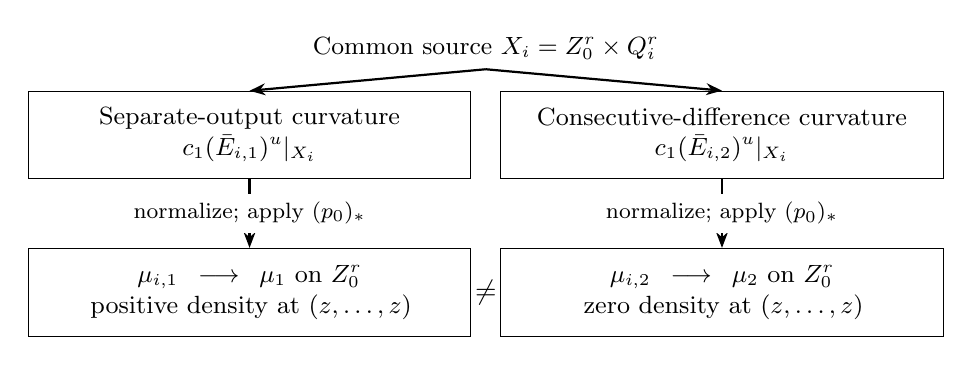
\begin{tikzpicture}[
  box/.style={draw,align=center,text width=5.2cm,
              inner sep=6pt,font=\small},
  arrow/.style={-{Stealth[length=2mm]},thick},
  note/.style={font=\footnotesize,align=center}]
\node[align=center,font=\small] (source) at (0,0)
  {Common source $X_i=Z_0^r\times Q_i^r$};
\node[box] (one) at (-3,-1.1)
  {Separate-output curvature\\$c_1(\bar E_{i,1})^u|_{X_i}$};
\node[box] (two) at (3,-1.1)
  {Consecutive-difference curvature\\$c_1(\bar E_{i,2})^u|_{X_i}$};
\draw[arrow] (source.south) -- (one.north);
\draw[arrow] (source.south) -- (two.north);
\node[box] (lowone) at (-3,-3.1)
  {$\mu_{i,1}\longrightarrow\mu_1$ on $Z_0^r$\\
   positive density at $(z,\ldots,z)$};
\node[box] (lowtwo) at (3,-3.1)
  {$\mu_{i,2}\longrightarrow\mu_2$ on $Z_0^r$\\
   zero density at $(z,\ldots,z)$};
\draw[arrow] (one) -- node[note,fill=white,inner sep=3pt]
  {normalize; apply $(p_0)_*$} (lowone);
\draw[arrow] (two) -- node[note,fill=white,inner sep=3pt]
  {normalize; apply $(p_0)_*$} (lowtwo);
\node at (0,-3.1) {$\ne$};
\end{tikzpicture}
\caption{The two curvature measures on the changing product $X_i$ are
normalized by their geometric degrees and projected to the fixed low
product $Z_0^r$. Their limits differ: a common nonzero low tangent vector
is killed by consecutive differences. If the arithmetic intersection
quotient $(\bar E_i^{d+1}\cdot Z_i)/(M_i^2B_i)$ tended to zero, uniform
metric variation would force these limits to agree. The smooth density
comparison gives the test function in \eqref{eq:low-measure-gap}.}
\label{fig:low-measures}
\end{figure}


\emph{Small points from a vanishing arithmetic intersection.}
We now suppose, contrary to the proposition, that the nonnegative
quotient in \eqref{eq:arithmetic-positive} tends to zero along a
subsequence.  We recall the two arithmetic inequalities used here and
in the small-section construction below.  For a nef adelic bundle
\(\bar D\) on a projective variety \(X\) of dimension \(n\), with
\(D\) geometrically big, the fundamental inequalities read
\begin{equation}\label{eq:fundamental-inequalities}
 \frac{e_1(X,\bar D)}{n+1}
 \le \frac{(\bar D^{n+1}\cdot X)}{(n+1)(D^n\cdot X)}
 \le e_1(X,\bar D).
\end{equation}
Here \(e_1\) is the essential minimum of the point height.  We use the
nef, geometrically big form of these inequalities
\cite[Theorem~5.3.3]{YuanZhang2021}; the ample projective case is
\cite[Theorem~1.10]{Zhang1995}.  We also use the arithmetic Siu inequality
\begin{equation}\label{eq:arithmetic-siu}
 \widehat{\operatorname{vol}}(\bar D-\bar N)
 \ge (\bar D^{n+1}\cdot X)
       -(n+1)(\bar D^n\bar N\cdot X)
\end{equation}
for nef adelic bundles, with the same absolute normalization
\cite[Theorem~A.5.1(2)]{YuanZhang2021}.
These statements apply after a projective resolution; pullback preserves
the intersection numbers and essential minima used here. Resolution in
characteristic zero can be performed over the original field \(k_i\),
by smooth-center blowups of a smooth projective ambient variety, with
centers disjoint from the original smooth locus of \(X\)
\cite[Theorems~1.0.2--1.0.3 and Section~5.7]{Wlodarczyk2005}.
Thus using a resolution
requires no extension of the bounded-degree field \(k_i\).  A bundle of
positive arithmetic volume has a nonzero section of some positive power
with supremum norm at most one at every place.  Its point height is
therefore nonnegative outside a proper closed subset.

By \eqref{eq:fundamental-inequalities} and
\eqref{eq:arithmetic-geometric-degrees}, each \(Z_i\) has a dense
set of points of \(\bar E_i\)-height at most \(\epsilon_iM_i^2\),
where \(\epsilon_i\to0\).  Products of these sets give a dense subset
\(\mathcal S_i\subset X_i(\Qbar)\) such that
\begin{equation}\label{eq:simultaneous-small-height}
 h_{\bar E_{i,1}}(x),\ h_{\bar E_{i,2}}(x)
 \le C_r\epsilon_iM_i^2\qquad(x\in\mathcal S_i).
\end{equation}
For the difference bundle this follows from
\(\|a-b\|^2\le2\|a\|^2+2\|b\|^2\).
We will use these common dense sets to show that, for every smooth real
function \(f\) on \(A_0^r(\mathbb C)\),
\begin{equation}\label{eq:low-measure-comparison}
 \mu_{i,1}(f)-\mu_{i,2}(f)\longrightarrow0.
\end{equation}
Applied to \(f_*\), this will contradict \eqref{eq:low-measure-gap}.
The required metric variation must be uniform in both the varieties and
their defining fields.

\emph{Uniform bounds for metric variation.}
Let \(v_i\) be the complex place of \(k_i\) determined by the chosen
embedding, and put \(\lambda_i=2/[k_i:\mathbb Q]\).  Thus
\(\lambda_i\) is bounded below by a positive constant.  Write
\(\overline{\mathcal O}_{v_i}(f)\) for the trivial bundle whose negative
logarithmic norm is \(p_0^*f\) at this embedding, its conjugate at the
conjugate embedding, and zero at all other places.  Write
\(\bar{\mathbf 1}\) for the trivial bundle with negative logarithmic
norm one at every archimedean place and zero at the finite places.
Its absolute point height is one.

Fix \(\eta>0\).  For either \(j\), abbreviate
\(\bar D_i=\bar E_{i,j}|_{X_i}\), \(\mu_i=\mu_{i,j}\), and set
\[
 a_i=\lambda_i\mu_i(f)-\eta,\qquad
 \bar U_i=\overline{\mathcal O}_{v_i}(f)-a_i\bar{\mathbf 1}.
\]
In particular \(|a_i|\le\|f\|_\infty+\eta\).  There are nef bundles
\(\bar U_{i,1},\bar U_{i,2}\), pulled back from the low ambient product,
such that
\begin{equation}\label{eq:uniform-nef-decomposition}
 \bar U_i=\bar U_{i,1}-\bar U_{i,2},\qquad
 \bar U_{i,2}=C\bar H+K\bar{\mathbf 1},
\end{equation}
where \(\bar H\) is a fixed canonical symmetric ample bundle on
\(A_0^r\), and \(C,K\) are fixed positive constants.  To obtain this,
choose an integer \(C\) so that
\(C c_1(\bar H)+dd^cf\) is semipositive, and then choose
\(K>\|f\|_\infty+\sup_i|a_i|\).

We spell out why this is nef in the model sense required by
\eqref{eq:arithmetic-siu}.  Start with a relatively ample projective model
of a power of \(H\), give it the invariant archimedean curvature, and
add a constant so that it is nef.  Normalized pullbacks by multiplication,
on graph models, converge to \(\bar H\); their archimedean curvatures
are all the same invariant form.  Adding the metric in
\eqref{eq:uniform-nef-decomposition} leaves every vertical curve degree
unchanged. At infinity the new curvature is semipositive by the choice
of \(C\). The added negative-log-norm function is nonnegative at each
archimedean place by the choice of \(K\), so the arithmetic degree of
every horizontal integral curve can only increase. This verifies the
nef criterion for hermitian models: semipositive curvature and
nonnegative degrees on all integral arithmetic curves. The perturbed
nef models converge to \(\bar U_{i,1}\).
The construction also applies to \(\bar U_{i,2}\), and its constants
are independent of \(i\) and of the field extension.

Every arithmetic mixed intersection of total order \(u+1\) formed from
\[
 \bar D_i,\qquad M_i^2\bar U_{i,1},\qquad M_i^2\bar U_{i,2}
\]
is bounded by
\begin{equation}\label{eq:uniform-mixed-intersections}
 O(M_i^2B_i^r),
\end{equation}
with one constant for all these finitely many types of intersections.
For a direct proof, let \(p_{a\ell}\) be the coordinate projection from
\(\cA^r\) to factor \(\ell\) in copy \(a\), and put
\[
 \bar T_i=\sum_{a=1}^r\sum_{\ell=0}^s
 b_{i\ell}^2p_{a\ell}^*\bar L_\ell,
 \qquad
 \bar S_i=\bar D_i+M_i^2\bar U_{i,1}
                 +M_i^2\bar U_{i,2}+\bar T_i
\]
on \(X_i\).  This is nef and geometrically ample.  Remove the factors
\(b_{i\ell}\) on each product tangent space.  The remaining forms
for \(D_i\) are bounded by \eqref{eq:scaled-homomorphisms}; those for
\(M_i^2U_{i,a}\) are bounded because their geometric parts use only
the low coordinates, where \(b_{i0}=M_i\).  Consequently
\[
 (S_i^u\cdot X_i)=O(B_i^r).
\]
On the products of the dense factorwise sets of height
\(O(H_{i\ell})\), all the point heights just displayed are
\(O(M_i^2)\).  For \(D_i\), use boundedness of \(\varphi_i\) to get
\[
 h_{\bar D_i}(x)\ll
 \sum_{a,\ell} b_{i\ell}^2
                 h_{\bar L_\ell}(x_{a\ell})=O(M_i^2).
\]
The same estimate holds for \(\bar T_i\).  The heights of
\(\bar U_{i,1},\bar U_{i,2}\) are bounded on these sets because the
low point heights and the metric shifts are bounded.  Thus
\(e_1(X_i,\bar S_i)=O(M_i^2)\), and the upper inequality in
\eqref{eq:fundamental-inequalities} yields
\((\bar S_i^{u+1}\cdot X_i)=O(M_i^2B_i^r)\).
Mixed intersections of nef adelic bundles are nonnegative.  Each term
in \eqref{eq:uniform-mixed-intersections} occurs with a positive
coefficient in this last self-intersection, which proves the assertion.
Absolute normalization has introduced no field-dependent constant.

\emph{Comparison against a low-factor test function.}
The metric intersection formula gives
\[
 (\bar D_i^u\bar U_i\cdot X_i)
 =(D_i^u\cdot X_i)\big(\lambda_i\mu_i(f)-a_i\big)
 =\eta(D_i^u\cdot X_i).
\]
Apply \eqref{eq:arithmetic-siu} to the two nef bundles
\(\bar D_i+tM_i^2\bar U_{i,1}\) and
\(tM_i^2\bar U_{i,2}\), where \(t>0\) is rational.  Expansion and
\eqref{eq:uniform-mixed-intersections} give
\begin{align*}
 \widehat{\operatorname{vol}}(\bar D_i+tM_i^2\bar U_i)
 \ &\ge (\bar D_i^{u+1}\cdot X_i)
 +(u+1)tM_i^2\eta(D_i^u\cdot X_i)
 -O(t^2M_i^2B_i^r).
\end{align*}
The first term is nonnegative.  By
\eqref{eq:arithmetic-geometric-degrees}, a sufficiently small fixed
\(t>0\), depending on \(f,\eta\) but not on \(i\), makes the right
side positive for all sufficiently large \(i\).  Hence the perturbed
height is nonnegative outside a proper closed subset of \(X_i\).

Repeat this argument for both \(j\) and for \(f\) and \(-f\).
Choose \(x_i\in\mathcal S_i\) outside the four resulting proper
closed subsets.  Let \(\operatorname{av}_{i,x_i}(f)\) be the average
of \(f\) on the low projections of the conjugates of \(x_i\) over
\(k_i\) at the chosen embedding.  Then
\[
 h_{\overline{\mathcal O}_{v_i}(f)}(x_i)
 =\lambda_i\operatorname{av}_{i,x_i}(f).
\]
Divide the perturbed height inequalities by \(tM_i^2\), and use
\eqref{eq:simultaneous-small-height}.  For \(j=1,2\) this yields
\[
 \left|\lambda_i\operatorname{av}_{i,x_i}(f)
             -\lambda_i\mu_{i,j}(f)\right|
 \le\eta+o(1).
\]
Since \(\inf_i\lambda_i>0\) and \(\eta\) is arbitrary, this proves
\eqref{eq:low-measure-comparison}.  This is the only point in this
metric-variation argument that needs the bounded degrees of the fields
\(k_i\); the degrees of the points \(x_i\) are unrestricted.

Taking \(f=f_*\) in \eqref{eq:low-measure-comparison} contradicts
\eqref{eq:low-measure-gap}.  This proves
\eqref{eq:arithmetic-positive}.
\end{proof}

\subsection{Sections with a uniform exponential bound}

The arithmetic intersection lower bound permits subtracting a constant
adelic bundle while keeping positive arithmetic volume.  Returning to
the original metric gives the following small sections over the fields
\(k_i\).

\begin{lemma}\label{lemma:small-sections}
For the products \(Z_i\), bundles \(\bar E_i\), and scalings above,
there is a constant \(c>0\) such that, for all sufficiently large
\(i\), a projective resolution \(\pi_i:\widetilde Z_i\to Z_i\)
over \(k_i\) carries a nonzero section defined over \(k_i\),
\[
 s_i\in H^0(\widetilde Z_i,\pi_i^*E_i^{\otimes n_i})
 \quad\text{for some integer }n_i>0
\]
whose adelic supremum norms satisfy
\begin{equation}\label{eq:small-section-norms}
 \|s_i\|_{v,\mathrm{sup}}\le
 \begin{cases}
 \exp(-cn_iM_i^2),&v\mid\infty,\\
 1,&v\nmid\infty.
 \end{cases}
\end{equation}
The resolution may be chosen to be an isomorphism over the smooth locus.
\end{lemma}

\begin{proof}
By Proposition~\ref{prop:arithmetic-positive} and
\eqref{eq:arithmetic-geometric-degrees}, there are constants
\(\delta,C>0\) with
\[
 (\bar E_i^{d+1}\cdot Z_i)\ge\delta M_i^2B_i,
 \qquad (E_i^d\cdot Z_i)\le CB_i.
\]
Choose \(0<c<\delta/((d+1)C)\).  The constant bundle
\(cM_i^2\bar{\mathbf 1}\) is nef, and
\eqref{eq:arithmetic-siu} shows that
\(\bar E_i-cM_i^2\bar{\mathbf 1}\) has positive arithmetic volume.
After pulling back to the resolution, take a nonzero section of a
positive power with norms at most one for this shifted metric.  Restoring
the original metric gives exactly \eqref{eq:small-section-norms}.
\end{proof}

The exponent \(n_i\) need not be bounded.  Its role is homogeneous:
the logarithmic norm bound is proportional to \(n_iM_i^2\), and the
weighted order in the next section is normalized by \(n_i b_{i\ell}^2\).
The fixed positive constant \(c\), together with
\(h_{\bar E_i}(y_i)=o(M_i^2)\), will force a positive weighted index
at the marked point.  Enlarging the field to calculate at that point
will not change the field of definition of the section.

\section{A uniform local index}
\label{sec:index}

The small sections constructed above vanish to a definite weighted order
at the marked points.  The essential issue is uniformity: the marked
points can have arbitrarily large degrees, and the coefficients of the
homomorphisms tend to infinity.  We prove the local assertion with these
two features explicit. The weighted Taylor-coefficient and Cauchy
argument follows the method of Faltings \cite[p.~560]{Faltings1991};
the estimates below supply the required uniformity for our varying
varieties and homomorphisms.

For a smooth point $y=(y_\ell)_\ell$ of a product
$Z=\prod_\ell Z_\ell$, choose regular parameters
$T_\ell=(T_{\ell,1},\ldots,T_{\ell,d_\ell})$ on each factor and a
local frame $e$ of a line bundle $E$.  If a nonzero section of $E^n$
has expansion $s=e^n\sum_\alpha a_\alpha T^\alpha$, define
\begin{equation}\label{eq:weighted-index}
 \operatorname{ind}_{n,b}(s;y)
 =\min_{a_\alpha\ne0}
       \sum_\ell\frac{|\alpha_\ell|}{n b_\ell^2}.
\end{equation}
A zero-dimensional factor contributes no parameters.  All parameters
in a given factor have the same weight.  Factorwise changes of regular
parameters preserve the corresponding filtration of the completed
local ring; multiplication by a unit also preserves its first nonzero
graded piece.  Thus the index is independent of these choices.

\begin{proposition}\label{prop:index}
Fix projective embeddings of abelian varieties $A_\ell$ by symmetric
very ample bundles $L_\ell$, a symmetric very ample canonically metrized
bundle $\bar L$ on $\cA=\prod_\ell A_\ell$, and integral bases of the
homomorphism groups between the fixed varieties.  Let
$F_i:\cA\to\cA$ be homomorphisms.  Suppose that:
\begin{enumerate}
\item $y_{i\ell}$ is a smooth point of an irreducible
$Z_{i\ell}\subset A_\ell$, its projective height is $O(H_{i\ell})$,
and its conormal space is spanned by equations of bounded degree and
coefficient height $O(H_{i\ell})$, with $H_{i\ell}\ge1$;
\item $M_i\longrightarrow\infty$, the positive integers $b_{i\ell}$
satisfy $b_{i\ell}\ll M_i$ and
$b_{i\ell}^2H_{i\ell}\asymp M_i^2$, and the coefficients of
$F_i|_{A_\ell}$ in the fixed bases are $O(b_{i\ell})$;
\item for $\bar E_i=F_i^*\bar L$ one has
$h_{\bar E_i}(y_i)=o(M_i^2)$, and a nonzero section $s_i$ of
$E_i^{n_i}$ on a resolution of $Z_i=\prod_\ell Z_{i\ell}$ satisfies
\begin{equation}\label{eq:index-small-section}
 \|s_i\|_{v,\sup}\le
 \begin{cases}
 e^{-c n_iM_i^2},&v\mid\infty,\\
 1,&v\nmid\infty,
 \end{cases}
\end{equation}
for a fixed $c>0$, over a number field containing its data.
\end{enumerate}
Assume that the resolution is an isomorphism over the smooth locus.
Then, for some $\eta>0$ independent of $i$,
$\operatorname{ind}_{n_i,b_i}(s_i;y_i)\ge\eta$ for all sufficiently
large $i$.  No bound on the degree of the field of $y_i$ is required.
\end{proposition}

\begin{proof}
For a first nonzero Taylor coefficient, Cauchy's inequality and the
product formula will compare the cost of differentiation,
\(\sum_\ell|\alpha_\ell|H_{i\ell}\), with the small-section gain
\(n_iM_i^2\).  The relation \(b_{i\ell}^2H_{i\ell}\asymp M_i^2\)
will turn this comparison into the asserted weighted index.  We first
choose the algebraic parameters and coefficient to which this argument
will apply, then bound the analytic radii and metric variation.

\emph{An algebraic coefficient and its local estimates.}
Enlarge the field of the section to a number field $E$ containing
$y_i$ and the equations to be used below.  At a place $v$ of $E$ write
$\nu_v=[E_v:\mathbb Q_{v|\mathbb Q}]/[E:\mathbb Q]$, with the usual
absolute values.  All heights and sums over places below use these
weights.  The constants do not depend on $[E:\mathbb Q]$.

Choose an affine projective-coordinate chart at $y_{i\ell}$.
From the equations in the first hypothesis choose a maximal invertible
Jacobian minor.  Center the coordinates at $y_{i\ell}$, write
$U_\ell$ for the coordinates in that minor and $T_\ell$ for the
remaining coordinates, and multiply the equations by the inverse
minor matrix.  They become
\begin{equation}\label{eq:index-implicit-system}
 U_\ell+\beta_\ell T_\ell+Q_\ell(T_\ell,U_\ell)=0,
\end{equation}
where $Q_\ell$ has no terms of degree less than two.  All degrees and
the number of coefficients are bounded.  Translation and matrix
inversion are bounded-degree rational operations on the original
coefficients and the affine point coordinates.  Consequently every
coefficient in \eqref{eq:index-implicit-system} has absolute height
$O(H_{i\ell})$.  Normalizing a nonzero coefficient of each original
equation to one justifies this assertion for coefficient vectors
initially specified only projectively.

Fix an algebraic local frame $e$, and a multi-index $\alpha$ attaining
\eqref{eq:weighted-index} in the factorwise parameters $T_\ell$ just
chosen.  If $a_\alpha$ is its coefficient, then
\[
 a_{\mathrm{fib}}=a_\alpha e(y_i)^{n_i}
       \in (E_i^{n_i})_{y_i}
\]
is a nonzero algebraic fiber element.  In any analytic frame its
coefficient times the value of that frame to the power $n_i$ equals
$a_{\mathrm{fib}}$.  Indeed a change of frame multiplies the
coefficient by its constant term, while all other contributions
involve coefficients of strictly smaller weighted order and vanish.
The multi-index is kept fixed here; only the index itself is asserted
to be independent of a change of parameters.

We will realize the parameters $T_\ell$ on analytic polydisks of radii
$\rho_{i\ell v}$ and choose analytic frames $e_v$ there.  If
\[
 \kappa_v=\sup_z\log\frac{\|e_v(y_i)\|_v}{\|e_v(z)\|_v},
\]
Cauchy's coefficient inequality, or its nonarchimedean Gauss-norm
counterpart, gives
\begin{equation}\label{eq:index-cauchy}
 \log\|a_{\mathrm{fib}}\|_v
 \le \log\|s_i\|_{v,\sup}+n_i\kappa_v
       +\sum_\ell|\alpha_\ell|\log\rho_{i\ell v}^{-1}.
\end{equation}
The estimate is first applied on smaller closed polydisks and then
passed to the indicated radii.  Because the left side uses the same
algebraic fiber element at every place, the product formula says
\[
 \sum_v\nu_v\log\|a_{\mathrm{fib}}\|_v
       =-n_i h_{\bar E_i}(y_i).
\]
It remains to bound the two losses on the right of
\eqref{eq:index-cauchy}: the inverse radii and the metric variation.

\emph{Analytic radii from the conormal equations.}
Let $S_{i\ell v}$ be the maximum of one and the absolute values of
the coefficients of \eqref{eq:index-implicit-system}.  Then
\begin{equation}\label{eq:index-coefficient-sum}
 \sum_v\nu_v\log S_{i\ell v}\ll H_{i\ell}.
\end{equation}
Fix tolerances $0<\gamma_v\le1$, determined by the place of a fixed
field of definition of the ambient data, equal to one outside its
infinite and finitely many finite places.  We may use the radii
\begin{equation}\label{eq:index-radii}
 \rho_{i\ell v}
 =\left(\frac{\gamma_v}{c_vS_{i\ell v}}\right)^4,
 \qquad
 \sum_v\nu_v\log\rho_{i\ell v}^{-1}\le C_\gamma H_{i\ell},
\end{equation}
where $c_v=1$ at finite places and a fixed sufficiently large constant
at infinite places.

Here is the analytic justification, including uniformity over
extensions.  At a finite place, on a smaller closed $T_\ell$-polydisk
of radius $s<\rho_{i\ell v}$, solve
$U=-\beta T-Q(T,U)$ in the Gauss-norm ball $\|U\|\le S_{i\ell v}s$.
The quadratic term has norm at most $S_{i\ell v}^3s^2$, and its
Lipschitz constant in $U$ is at most $S_{i\ell v}^2s<1$.
The map therefore preserves the ball and is a contraction.
At an infinite place use instead the ball
$\|U\|\le C_1S_{i\ell v}s$, with a fixed $C_1$ larger than twice the
maximum number of entries in a row of $\beta_\ell$. This absorbs the
row sums in its linear term. Bounds for the quadratic term and its
Lipschitz constant now acquire only fixed factors depending on $C_1$,
the degrees and the number of monomials. Increasing $c_v$ makes the
quadratic contribution smaller than half the ball radius and makes the
Lipschitz constant less than one.  The solutions for smaller disks agree and give an
analytic parametrization on the open polydisk of radius
$\rho_{i\ell v}$.  All affine coordinate displacements have norm
less than $\gamma_v$, and the Jacobian in $U$ remains invertible.
At the center these equations define the germ of $Z_{i\ell}$:
they define a smooth complete intersection of its dimension containing
that germ.  Every further equation of $Z_{i\ell}$ thus vanishes as
a power series after substitution, and hence on the whole analytic
branch.  The invertible minor shows that this branch remains in the
smooth locus.  Finally \eqref{eq:index-coefficient-sum} gives the
second assertion of \eqref{eq:index-radii}.  Notice that sums of
weights over the places above a fixed place do not change under
extension of $E$.

\emph{Metric variation at the infinite places.}
We next choose the tolerances so that the metric varies little on the
product of these branches.  At infinity, fix a small $\xi>0$.
The bound on affine coordinate displacements gives a uniform bound
on projective distance: for $x=[1:a]$ and $x'=[1:a+u]$, the chordal
distance is at most a fixed constant times $\|u\|$, because both
homogeneous coordinate norms are at least one. Compactness of the fixed
complex abelian varieties and local exponential charts therefore allow
us to make each group difference from the center have an analytic
logarithm of norm at most $\xi$.  Its image
under $F_i$ has a logarithmic lift of norm
$O(\xi\sum_\ell b_{i\ell})=O(\xi M_i)$.  The same coefficient
bound holds at every infinite embedding: all norms on the fixed
finite-dimensional real homomorphism spaces are comparable.

On the target universal cover, centered at a lift of $F_i(y_i)$,
the canonical curvature has a fixed quadratic potential $Q$.
There is a holomorphic frame $e_v$ whose negative log norm differs
from its value at the origin by $Q$: subtracting this potential
leaves a flat metric, with a unitary holomorphic frame on the simply
connected cover.  Pull this frame back along the logarithmic lift
of our polydisk.  We obtain
\begin{equation}\label{eq:index-infinite-metric}
 \sup_z\log\frac{\|e_v(y_i)\|_v}{\|e_v(z)\|_v}
 \le C\xi^2M_i^2.
\end{equation}
The constant is independent of the center.  The image of the polydisk
need not lie in an injectivity neighborhood on the target: the
construction takes place on its universal cover.

\emph{Metric variation at the finite places.}
At a finite place we need a different estimate, independent of all
integer coefficients of $F_i$.  Outside a fixed finite set of places,
the varieties, group laws, polarization data and basis homomorphisms
extend over good models.  Differences of reduction zero remain of
reduction zero under every integral linear combination of the basis
homomorphisms.  The choice $\gamma_v=1$ therefore suffices there.

At one of the remaining places, work over the completed algebraic
closure.  Arbitrarily small analytic balls at the identity are
subgroups.  Indeed, in fixed smooth group parameters addition is
$u+v$ plus terms of degree at least two, and inversion is $-u$ plus
terms of degree at least two; on a sufficiently small ball the
nonarchimedean inequality makes both operations preserve that ball.
In particular the ball is stable under multiplication by every
integer.  Choose a target subgroup ball small enough that translation
by any of its points preserves the reduction class in the fixed
projective embedding.  Such a choice is uniform in the point being
translated.  Here is a uniform projective estimate for this assertion. For normalized
homogeneous coordinates, write
\[
 d_v(x,x')=\frac{\max_{a,b}|x_ax'_b-x_bx'_a|_v}
                  {\max_a|x_a|_v\max_a|x'_a|_v}.
\]
In a common affine chart, coordinate displacements of norm less than
$\gamma_v\le1$ imply $d_v(x,x')<\gamma_v$, even when the affine
coordinates of the center are unbounded. A fixed projective morphism $f$
has finitely many homogeneous polynomial presentations which together
have no base point on its source. A homogeneous Nullstellensatz
identity gives a fixed $\varepsilon_v>0$ such that at every normalized
source point one presentation has value of norm at least $\varepsilon_v$. Polynomial
difference estimates give a fixed $C_v'$ such that, when
$d_v(x,x')$ is below a fixed threshold, the same presentation remains
nonzero and
\[
 d_v(f(x),f(x'))\le C_v' d_v(x,x').
\]
To apply the polynomial estimate, rescale nearby normalized coordinate
vectors so that their coordinate differences are bounded by their
projective distance; this is possible in a coordinate which is a unit
at both points. All constants are in the fixed coefficient field and
remain valid over its completed algebraic closure.
Apply the estimate to the difference morphism and to translation
$A\times A\to A$, comparing $(a,b)$ with $(a,0)$. Thus the source
coordinate tolerances uniformly control identity neighborhoods, and
translation by a sufficiently small identity neighborhood preserves
projective reduction for every center.

The finitely many basis homomorphisms carry sufficiently small source
identity neighborhoods into this target subgroup ball.  Every integral
linear combination does so too.  We can therefore choose the input
tolerances $\gamma_v$ independently of $i$ so that the target remains
in the reduction class of $F_i(y_i)$ throughout the product branch.
A homogeneous coordinate having maximal absolute value at this center
defines a nonvanishing frame with constant projective metric norm on
the branch.  The comparison between this metric and the canonical
metric gives
\begin{equation}\label{eq:index-finite-metric}
 \sup_z\log\frac{\|e_v(y_i)\|_v}{\|e_v(z)\|_v}\le C_v,
 \qquad \sum_{v\nmid\infty}\nu_v C_v\le C_0,
\end{equation}
where $C_v=0$ outside the fixed bad places.  These constants remain
unchanged upon extension of the point field.  This is the step that
prevents a loss depending on the sizes of the integers in $F_i$.

\emph{Summing over the places.}
The constructed frames satisfy $\kappa_v\le C\xi^2M_i^2$ at infinity
and $\kappa_v\le C_v$ at finite places.  The section norm bound applies
on all the branches because they lie in the resolution's isomorphic
smooth locus.  Sum \eqref{eq:index-cauchy}, using the product formula,
the small-section bound \eqref{eq:index-small-section}, the radius
estimate \eqref{eq:index-radii}, and the two metric estimates
\eqref{eq:index-infinite-metric} and \eqref{eq:index-finite-metric}.  We
obtain
\[
 C_\gamma\sum_\ell|\alpha_\ell|H_{i\ell}
 \ge n_i\bigl((c-C\xi^2)M_i^2-C_0-o(M_i^2)\bigr).
\]
Choose $\xi$ so that $C\xi^2<c/2$, then let $i$ tend to infinity.
The comparison $b_{i\ell}^2H_{i\ell}\asymp M_i^2$ now yields a
fixed positive lower bound for \eqref{eq:weighted-index}.
\end{proof}

For the products chosen in Proposition~\ref{prop:minimal-products},
the first hypothesis is precisely its smoothness and equation
conclusion.  The homomorphisms and weights of
Section~\ref{sec:arithmetic} satisfy the second hypothesis;
\eqref{eq:small-marked-height} and
Lemma~\ref{lemma:small-sections} give the third.  We therefore have
a fixed positive index at $y_i$.  The next section converts it into
a hypersurface of bounded degree over a field of bounded degree,
which is the contradiction required by minimality.

\section{The product cut and bounded-degree descent}
\label{sec:product-cut}

The positive index from Proposition~\ref{prop:index} will produce a
hypersurface containing some $y_{i\ell}$ but not $Z_{i\ell}$.
Both its degree and
the degree of a field of definition must be bounded: geometric degree
alone would not contradict Proposition~\ref{prop:minimal-products}.
We first transfer the section to a polynomial on a product of
projective spaces, and then keep track of all conjugates of a suitable
component of its index locus.

\subsection{Finite projections and the norm of a section}

The section $s_i$ supplied by Lemma~\ref{lemma:small-sections} is
defined over $k_i$.  The larger field used in the local index proof
serves only to evaluate this section and its coefficients at the
marked point; it does not change the section's field of definition.

Choose a fixed positive integer $t_0$ such that
\begin{equation}\label{eq:cut-ample-difference}
 Q_i=t_0\sum_\ell b_{i\ell}^2L_\ell-F_i^*L
\end{equation}
is ample on $\cA$.  This is possible uniformly in $i$: after changing
variables by $\operatorname{diag}(b_{i\ell})$ in the invariant
Hermitian forms, the first term is a fixed positive form times $t_0$,
whereas the second is bounded because
$F_i\operatorname{diag}(b_{i\ell}^{-1})$ is bounded.

Take a positive power making $Q_i$ globally generated.  Replacing
$s_i$ by the corresponding power, and $n_i$ by the same multiple,
choose a section of $Q_i^{n_i}$ over $k_i$ nonzero at $y_i$ and
multiply.  Such a section exists over $k_i$: among a $k_i$-basis of
a generating space, some member has nonzero value at the algebraic
point $y_i$.  We obtain a nonzero section $s'_i$ of
\[
 \left.\boxtimes_\ell L_\ell^{t_0n_ib_{i\ell}^2}\right|_{Z_i}
\]
on the resolution.  Its index with weights $n_ib_{i\ell}^2$ is still
at least the fixed constant of Proposition~\ref{prop:index}; taking
a power scales numerator and denominator together, and multiplication
by a regular section cannot lower weighted order.

Let $Z_i^\nu$ be the normalization of $Z_i$.  The proper
birational map from the resolution to $Z_i^\nu$ has
pushforward structure sheaf $\mathcal O_{Z_i^\nu}$.  The
projection formula therefore descends $s'_i$ to the pullback of the
displayed bundle on $Z_i^\nu$.  We do not require descent to
the possibly nonnormal variety $Z_i$ itself.

For each factor choose a finite linear projection
\[
 \pi_{i\ell}:Z_{i\ell}\longrightarrow\mathbb P^{d_\ell},
 \qquad \pi_{i\ell}^*\mathcal O(1)=L_\ell|_{Z_{i\ell}},
\]
which is \'{e}tale at $y_{i\ell}$.  A general projection has this
property at a specified smooth point.  The same requirements at its
finitely many conjugates give a nonempty open condition defined over
$k_i$ in the space of projections.  Since $k_i$ is infinite, it
contains a choice over $k_i$.  The degree of this finite map is
$\deg_{L_\ell}Z_{i\ell}$ and is bounded.  A zero-dimensional
geometrically integral factor defined over $k_i$ is a $k_i$-point;
its projection to $\mathbb P^0$ has degree one.

The product projection, composed with normalization, is a finite map
\[
 \Pi_i:Z_i^\nu\longrightarrow
            P_i=\prod_\ell\mathbb P^{d_\ell}
\]
of bounded degree
$e_i=\prod_\ell\deg_{L_\ell}Z_{i\ell}$.
Take the field norm of $s'_i$ along this map, as in
\cite[p.~565]{Faltings1991}.  It is a nonzero
section $G_i$ on $P_i$, defined over $k_i$, with multidegrees
\begin{equation}\label{eq:cut-multidegrees}
 D_{i\ell}=e_it_0n_ib_{i\ell}^2.
\end{equation}
For completeness, on an affine trivializing open of the target,
$s'_i$ is an element of a finite algebra over the coordinate ring.
It is integral there; the coefficients of its characteristic
polynomial in the function-field extension are integral and belong
to the fraction field of the normal target ring, and hence belong
to that ring.  Thus its norm is regular.  On overlaps, a change of
frame is raised to the power $e_i$, proving
\eqref{eq:cut-multidegrees}.  This also proves that the construction
works without a flatness hypothesis for $\Pi_i$.

The characteristic polynomial shows that the pullback of $G_i$ is
divisible by $s'_i$ in the local ring at $y_i$.  Because the
projections are \'{e}tale factor by factor there, their completed local
rings over $\Qbar$ identify through factorwise parameters.  If
$z_i=\Pi_i(y_i)$, it follows that
\begin{equation}\label{eq:cut-polynomial-index}
 \operatorname{ind}_{D_i}(G_i;z_i)\ge\eta_1>0,
\end{equation}
where $\operatorname{ind}_{D_i}$ gives parameters in the $\ell$th
projective factor weight $D_{i\ell}^{-1}$.  Indeed the change from
the old weights divides the index by $e_it_0$, which is bounded.
We now omit the zero-dimensional projective factors.  At least one
factor remains because $d_0>0$.  For the remaining ordered factors,
\begin{equation}\label{eq:cut-ratios}
 D_{i\ell}/D_{i,\ell+1}\longrightarrow\infty,
\end{equation}
including when omitted factors occur between them.

\subsection{Components of separated index loci}

Let $G$ be a nonzero multihomogeneous polynomial of positive
multidegrees $D=(D_1,\ldots,D_m)$ on
$P=\prod_{\ell=1}^m\mathbb P^{d_\ell}$, with $d_\ell\ge1$, and write
$N=\sum_\ell d_\ell$.  Its index at a point is the minimum of
$\sum_\ell|\alpha_\ell|/D_\ell$ among nonzero coefficients in
local affine coordinates and a local frame.  Equivalently one may
use homogeneous partial derivatives, with their total orders in
each block as weights.  This equivalence follows by dehomogenizing
in a nonzero coordinate: affine derivatives are homogeneous
derivatives divided by the local frame, while derivatives in the
omitted coordinate are combinations of affine derivatives of no
larger weighted order, by homogeneity.

For a positive irrational number $\sigma$, let $\mathcal I_\sigma$
be the closed locus where this index exceeds $\sigma$.  It is cut
out by all homogeneous derivatives having weighted order less than
$\sigma$.  All occurring weights are rational, so changing either
strict inequality to a nonstrict one gives the same locus.

Suppose that $z\in P$ has index at least $\eta>0$.  Following
\cite[Remark~3.4]{Faltings1991}, we first find a component through $z$
that persists between two separated levels.
Choose a positive irrational $\sigma_0$ and a positive rational
$\epsilon\le1$ such that the $N+2$ levels
\[
 \sigma_j=\sigma_0+j\epsilon\qquad(0\le j\le N+1)
\]
all lie below $\eta$.  These choices depend only on $\eta$ and $N$,
not on the multidegrees $D$.  The point $z$ lies in every corresponding
index locus.  Choose a component $J_{N+1}$ through $z$ at the highest
level and then, at each lower level, a component containing the one
already chosen.  This gives
\[
 J_{N+1}\subseteq J_N\subseteq\cdots\subseteq J_0,
 \qquad J_j\text{ a component of }\mathcal I_{\sigma_j}.
\]
Every $J_j$ is proper in $P$, because $G\ne0$ and all levels are
positive.  Two consecutive components coincide: otherwise their
dimensions would strictly increase more than $N$ times.  Their common
value $J$ contains $z$ and is a component of both
$\mathcal I_\sigma$ and $\mathcal I_{\sigma+\epsilon}$ for one of
the chosen levels $\sigma$.

We use Faltings' product theorem \cite[Theorem~3.1]{Faltings1991}
in Evertse's explicit form:
for $m\ge2$, $0<\epsilon\le1$, and
\begin{equation}\label{eq:cut-product-threshold}
 D_\ell/D_{\ell+1}\ge(mN/\epsilon)^N,
\end{equation}
a common irreducible component of the index loci at levels
$\sigma$ and $\sigma+\epsilon$ is a product of subvarieties of the
individual projective factors.  This is
\cite[Theorem~1]{Evertse1995Product}, an explicit version of
Faltings' theorem; its hypotheses concern a nonzero polynomial over
an algebraically closed field of characteristic zero.  Thus, over
$\Qbar$, the component just constructed is a product whenever
\eqref{eq:cut-product-threshold} holds.  For $m=1$ it is already a
subvariety of the single projective factor.

It remains to bound both the factor degrees and a common field of
definition independently of $D$.  Evertse's theorem also gives such
an arithmetic bound.  The next lemma proves the needed weaker bound
directly by Faltings' conjugate-counting method
\cite[Remark~3.2]{Faltings1991}, including the case $m=1$.

\begin{lemma}\label{lemma:conjugate-product-degree}
Suppose that $G$ is defined over a number field $k$, and that a
proper geometric component
$J=\prod_{\ell=1}^mJ_\ell$ is common to
$\mathcal I_\sigma$ and $\mathcal I_{\sigma+\epsilon}$, where
$\sigma>0$ and $0<\epsilon\le1$, and neither level is a rational
derivative weight.  If $q$ is the number of conjugates of $J$ over
$k$, then
\begin{equation}\label{eq:conjugate-product-degree}
 q\prod_\ell\deg J_\ell\le C(N,\epsilon).
\end{equation}
In particular the factors have bounded degrees and are defined over
a common extension of $k$ of bounded degree.
\end{lemma}

\begin{proof}
Put $c_\ell=\codim_{\mathbb P^{d_\ell}}J_\ell$ and
$c=\sum_\ell c_\ell>0$.  Both index loci are defined over $k$, so
every conjugate of $J$ is again a common component.  All conjugates
have the same factor codimensions.  Choose general linear spaces
$\Lambda_\ell\simeq\mathbb P^{c_\ell}$ and put
$\Lambda=\prod_\ell\Lambda_\ell$.  Each conjugate of $J$ meets
$\Lambda$ transversely in $\prod_\ell\deg J_\ell$ reduced points.
We may choose the slices so that all these sets are disjoint and
none of their points belongs to any other component of
$\mathcal I_\sigma$.

Here is the incidence justification for this simultaneous choice.
The intersection of a component $J'$ with another component of
$\mathcal I_\sigma$ is a proper closed subset of $J'$, hence has
dimension less than $\dim J'$.  For a fixed point, the condition
that it belong to $\Lambda$ has codimension
$\sum_\ell(d_\ell-c_\ell)=\dim J'$ in the product of the
Grassmannians parametrizing the slices.  Thus a general product
slice misses every such proper subset.  There are only finitely
many components and conjugates.  The same argument, together with
generic transversality in each factor in characteristic zero,
avoids the singular loci.  It follows that the indicated
$q\prod_\ell\deg J_\ell$ points are isolated in
$\Lambda\cap\mathcal I_\sigma$.  They all belong to the higher
index locus.

Multiply each derivative defining $\mathcal I_\sigma$ by all
monomials of the missing multidegree, so that every resulting
equation has multidegree $D$.  This operation does not change their
common zero set: at any point, some monomial of each specified
nonnegative multidegree is nonzero.  Near a point of the higher
index locus, differentiating by weighted order less than $\sigma$
leaves weighted order at least $\epsilon$.  Multiplying by a
monomial cannot lower this order.  Restriction to $\Lambda$ is
factorwise and cannot lower it either.

Choose $c$ general linear combinations of these restored equations
so that their restrictions to $\Lambda$ have isolated intersections
at every indicated point.  This is possible because the common
base locus is isolated there: successive general combinations avoid
the finitely many associated components of positive dimension
through these finitely many points.  In completed local coordinates
$t_{\ell,1},\ldots,t_{\ell,c_\ell}$ at one such point, their
ideal is contained in the monomial ideal generated by monomials of
weighted order at least $\epsilon$.  The local intersection
multiplicity is therefore at least the number of monomials of
weight less than $\epsilon$.

In particular consider monomials for which every exponent in the
$\ell$th block is strictly less than $\epsilon D_\ell/(2c)$.
Their total weight is less than $\epsilon/2$, and their number is
at least
\begin{equation}\label{eq:cut-local-multiplicity}
 \left(\frac{\epsilon}{2c}\right)^c
       \prod_\ell D_\ell^{c_\ell}.
\end{equation}
Indeed there are $\lceil x\rceil\ge x$ nonnegative integers
strictly less than a positive real number $x$.

On the other hand, the sum of the isolated intersection
multiplicities of $c$ divisors of multidegree $D$ on $\Lambda$ is
at most
\begin{equation}\label{eq:cut-bezout}
 \left(\sum_\ell D_\ell H_\ell\right)^c\cdot\Lambda
 =\frac{c!}{\prod_\ell c_\ell!}\prod_\ell D_\ell^{c_\ell},
\end{equation}
where $H_\ell$ denotes the hyperplane class from the $\ell$th
factor.  The bound remains valid if other intersection components
have positive dimension.  Namely, perturb the divisors in their
basepoint-free complete linear systems to make the intersection
proper; at each original isolated complete intersection the local
length is conserved, and its contribution is part of the total
degree \eqref{eq:cut-bezout}.  There are
$q\prod_\ell\deg J_\ell$ of the isolated points counted above.
Combining their individual multiplicity bound with the total bound gives
\[
 q\left(\prod_\ell\deg J_\ell\right)
   \left(\frac{\epsilon}{2c}\right)^c
   \prod_\ell D_\ell^{c_\ell}
 \le \frac{c!}{\prod_\ell c_\ell!}
       \prod_\ell D_\ell^{c_\ell}.
\]
The powers of the multidegrees cancel, proving
\eqref{eq:conjugate-product-degree} independently of $D$.
For example, after harmless enlargement the constant is bounded by
$N!(2N/\epsilon)^N$.

Finally, the stabilizer of $J$ in the absolute Galois group of $k$
has index $q$.  Galois descent defines $J$ over its fixed field,
a degree-$q$ extension of $k$.  Each $J_\ell$ is the image of $J$
under a factor projection, so it is defined over the same field.
All factor degrees are positive integers; hence
\eqref{eq:conjugate-product-degree} bounds them separately as well.
\end{proof}

\subsection{The contradiction to minimality}

\begin{proposition}\label{prop:product-cut}
For the minimal products of Proposition~\ref{prop:minimal-products}
with $d_0>0$, the small sections of
Lemma~\ref{lemma:small-sections} cannot satisfy the positive index
conclusion of Proposition~\ref{prop:index} along an infinite
subsequence.
\end{proposition}

\begin{proof}
The finite projections and norms above give $G_i$ and $z_i$ with
\eqref{eq:cut-polynomial-index}.  Pass to constant dimensions of
the projective factors and let $N$ be their sum.  Apply the preceding
component construction with $\eta=\eta_1$.  Its $N+2$ levels and their
gap $\epsilon$ are fixed independently of $i$.  It gives a proper
component $J_i$ through $z_i$ common to two adjacent index loci;
the adjacent pair may depend on $i$.

For at least two factors, \eqref{eq:cut-ratios} eventually implies
\eqref{eq:cut-product-threshold}, so the product theorem gives
$J_i=\prod_\ell J_{i\ell}$.  With one factor this conclusion
requires no theorem.  Lemma~\ref{lemma:conjugate-product-degree}
then gives a common field of definition $k_i'$ with
$[k_i':k_i]$ bounded and all $\deg J_{i\ell}$ bounded.
The finitely many possible choices of adjacent levels do not
affect these bounds.

Because $J_i$ is proper, at least one factor $J_{i\ell}$ is
proper in $\mathbb P^{d_\ell}$.  After extraction fix this index
$\ell$.  A proper projective variety of bounded degree admits a
nonzero homogeneous equation of bounded degree over its field of
definition.  One can obtain it by projecting generally over that
field to a hypersurface in a projective space of one larger
dimension than the variety and pulling back its equation; the
image degree does not exceed the original degree.  Let $R_i$ be
such an equation for $J_{i\ell}$ over $k_i'$.

Pulling back $R_i$ through the linear projection $\pi_{i\ell}$
gives a bounded-degree hypersurface over $k_i'$ containing
$y_{i\ell}$.  It does not contain $Z_{i\ell}$, because that
projection is surjective onto $\mathbb P^{d_\ell}$ and $R_i$ is
nonzero.  The degrees $[k_i':\mathbb Q]$ are bounded, since the
degrees $[k_i:\mathbb Q]$ were bounded in choosing the minimal
products.  This is exactly the hypersurface excluded by
Proposition~\ref{prop:minimal-products}, a contradiction.
\end{proof}

\begin{proof}[Completion of the proof of Theorem~\ref{thm:sequence}]
Theorem~\ref{thm:all-high} handles the case with only unbounded
scales.  For a counterexample with a low factor, choose one of
minimal ambient dimension.  The projection and tangent arguments
apply in this minimal counterexample.  Proposition~\ref{prop:minimal-products}
then provides its auxiliary products.  If $d_0=0$,
Lemma~\ref{lemma:fixed-low-point} produces an all-high
counterexample, already impossible.  If $d_0>0$,
Proposition~\ref{prop:arithmetic-positive} and
Lemma~\ref{lemma:small-sections} provide the small sections;
Proposition~\ref{prop:index} gives their positive index; and
Proposition~\ref{prop:product-cut} contradicts minimality of the
auxiliary products.  Thus there is no counterexample with a low
factor either.
\end{proof}

\section{From non-density to maximal atypical finiteness}\label{sec:finiteness}

The sequence theorem and its reduction in Section~\ref{sec:sequences}
prove Theorem~\ref{thm:nondensity} for every abelian variety over $\Qbar$.
We now explain why this universal statement gives the finiteness
asserted in Theorem~\ref{thm:main}. We use the reduction of Barroero
and Dill \cite[Theorem~1.9]{BarroeroDill2021}; their passage from
optimal points to positive-dimensional optimal subvarieties uses
Habegger and Pila's \cite[Theorem~9.8(i)]{HabeggerPila2016}.

For an irreducible subvariety $Z$ of an abelian variety, its
\emph{special defect} is
\[
 \delta(Z)=\dim\langle Z\rangle_{\mathrm{sp}}-\dim Z.
\]
An irreducible $Z\subseteq X$ is \emph{optimal in $X$} if every
irreducible $U$ with $Z\subsetneq U\subseteq X$ satisfies
$\delta(U)>\delta(Z)$. This uses special closure, in contrast to the
arbitrary-coset closure used for geodesic optimality in
Section~\ref{sec:tangent}.

\begin{proposition}\label{prop:optimal-finite}
Every irreducible subvariety of every abelian variety over $\Qbar$
contains only finitely many optimal subvarieties.
\end{proposition}

\begin{proof}
Fix an abelian variety $A$, and nonnegative integers $m,e$.
Theorem~1.9 of \citet{BarroeroDill2021} has the following implication.
Suppose that, for every abelian subvariety $B\subseteq A$ and every
irreducible $Z\subseteq B$ of dimension at most $m$ which is not
contained in a proper special subvariety of $B$, the set
\[
 Z\cap B^{[\max\{\dim Z+1,\,\dim B-e\}]}
\]
is not dense in $Z$. Then each irreducible subvariety of $A$ of
dimension at most $m$ has only finitely many optimal subvarieties of
defect at most $e$.

The displayed intersection is a subset of
$Z\cap B^{[\dim Z+1]}$, so Theorem~\ref{thm:nondensity} verifies the
hypothesis for every $B$ and $Z$ in this statement. All these varieties
are defined over number fields after finite extension. The same
non-density theorem is available for quotients and isogenous varieties
as well, so no ambient restriction is introduced by the reduction.
Take $m=\dim X$ and $e=\dim A$. Every special defect in $A$ lies between
$0$ and $\dim A$, which proves the proposition.
\end{proof}

\begin{lemma}\label{lem:maximal-optimal}
Let $X$ be an irreducible subvariety of an abelian variety and
$S=\langle X\rangle_{\mathrm{sp}}$. Every maximal atypical subvariety
of $X$ in $S$ is optimal in $X$.
\end{lemma}

\begin{proof}
Let $Y$ be maximal atypical, witnessed by a special $T\subseteq S$.
Since $\langle Y\rangle_{\mathrm{sp}}\subseteq T$, inequality
\eqref{eq:atypical} gives
\[
 \delta(Y)\le\dim T-\dim Y
 <\dim S-\dim X=\delta(X).
\]
Suppose $Y\subsetneq U\subseteq X$ and
$\delta(U)\le\delta(Y)$. Put $T'=\langle U\rangle_{\mathrm{sp}}$;
then $T'\subseteq S$ by \eqref{eq:closure-monotonicity}.
Choose an irreducible component $C$ of $X\cap T'$ containing $U$.
We have
\[
 \dim C\ge\dim U
 =\dim T'-\delta(U)
 >\dim T'-\delta(X)
 =\dim X+\dim T'-\dim S.
\]
Thus $C$ is atypical and strictly contains $Y$, a contradiction.
\end{proof}

\begin{proof}[Proof of Theorem~\ref{thm:main}]
Write $S=B+\tau$ with $\tau$ torsion. Translation by $-\tau$ identifies
$S$ with the abelian variety $B$, preserves dimensions and special
subvarieties, and sends $X$ to a subvariety with special closure $B$.
The torsion point, $B$ and this translated subvariety are all defined
over a number field after a finite extension. We may therefore work
inside $B$.

Proposition~\ref{prop:optimal-finite} and
Lemma~\ref{lem:maximal-optimal} show that the set of maximal atypical
subvarieties is finite. Each is proper: if $X$ were a component
witnessing its own atypicality, the witnessing special subvariety
would contain $X$ and hence equal its special closure, making the
strict dimension inequality impossible. Starting from any atypical
subvariety, a sequence of strict atypical enlargements increases
dimension and must terminate. Thus every atypical subvariety lies in a
maximal one. Their finite union is a proper closed subset of the
irreducible variety $X$.

If $\dim X=0$, a special subvariety containing its only point must
contain its special closure, so there are no atypical subvarieties.
This also covers the zero-dimensional ambient case. The assertions
and the possibility of an empty exceptional list follow in every case.
\end{proof}

\section{Finite-rank translated intersections}\label{sec:finite-rank}

We derive Corollary~\ref{cor:finite-rank-translates} from
Theorem~\ref{thm:nondensity} by Pink's reduction
\cite[Theorem~5.3]{Pink2005}, which extends an argument of
R\'emond and Viada \cite[Proposition~4.2]{RemondViada2003} from powers
of an elliptic curve to semiabelian varieties.  The auxiliary ambient
group constructed below is again an abelian variety over $\Qbar$.

For an abelian variety $V$ and an integer $r\ge0$, the set
$V^{[r]}(\Qbar)$ is also the union of $G(\Qbar)$ over all algebraic
subgroups $G\subseteq V$ of codimension at least $r$. Indeed, every
irreducible component of an algebraic subgroup is a torsion coset of
the same dimension. Conversely, a torsion coset $D+\tau$ is contained
in the algebraic subgroup $D+\langle\tau\rangle$, which has dimension
$\dim D$ because $\tau$ is torsion. Thus this notation agrees with the
algebraic-subgroup union used in Pink's reduction.

\begin{proof}[Proof of Corollary~\ref{cor:finite-rank-translates}]
Put $r=\dim_{\mathbb Q}(\Gamma\otimes_{\mathbb Z}\mathbb Q)$ and choose
$a_1,\ldots,a_r\in\Gamma$ whose images form a basis of this vector
space. Let $D\subseteq A^r$ be the Zariski closure of the subgroup
generated by $(a_1,\ldots,a_r)$. Choose a positive integer $m$ that
annihilates the finite component group $D/D^0$. Multiplication by $m$
is surjective on the abelian variety $D^0$, so $[m]D=D^0$. It is also
a finite, hence closed, morphism on $A^r$. Consequently
\[
 \overline{\langle (ma_1,\ldots,ma_r)\rangle}=[m]D=D^0.
\]
Replace each $a_i$ by $ma_i$, write $a=(a_1,\ldots,a_r)$, and put
$C=D^0$. The images of the new $a_i$ still form a basis of
$\Gamma\otimes_{\mathbb Z}\mathbb Q$, and the cyclic subgroup generated
by $a$ is Zariski dense in the connected abelian subvariety $C$.
When $r=0$, this construction uses the empty tuple and the zero abelian
variety. For every $\gamma\in\Gamma$ there are integers $n>0$ and
$n_1,\ldots,n_r$ such that
\begin{equation}\label{eq:finite-rank-relation}
 n\gamma=n_1a_1+\cdots+n_ra_r.
\end{equation}
Indeed, a relation after tensoring with $\mathbb Q$ has only a torsion
error, which a further positive multiple kills.

Set $B=A\times C$ and $Y=X\times\{a\}$. Both are defined over $\Qbar$;
$B$ is abelian and $Y$ is irreducible of dimension $d$. We check that
$Y$ is contained in no proper algebraic subgroup of $B$. If an
algebraic subgroup $J\subseteq B$ contains $Y$, fix $x_0\in X(\Qbar)$.
Then $J$ contains $(x-x_0,0)$ for every $x\in X(\Qbar)$. The Zariski
closure of the subgroup of $A$ generated by these differences is all of
$A$: otherwise its translate by $x_0$ would be a proper translate
containing $X$.
It follows that $A\times\{0\}\subseteq J$. The projection of $J$ to
$C$ is a closed algebraic subgroup containing $a$, and hence is $C$.
These two facts imply $J=B$. Since every proper torsion coset lies in a
proper algebraic subgroup of the same dimension, $Y$ is contained in
no proper torsion coset. Theorem~\ref{thm:nondensity} therefore shows
that $Y(\Qbar)\cap B^{[d+1]}(\Qbar)$ is not Zariski dense in $Y$.

It remains to verify the inclusion
\begin{equation}\label{eq:finite-rank-inclusion}
 \bigl(X(\Qbar)\cap(A^{[d+1]}(\Qbar)+\Gamma)\bigr)\times\{a\}
 \subseteq Y(\Qbar)\cap B^{[d+1]}(\Qbar).
\end{equation}
Let $x=g+\gamma$ belong to the intersection on the left, with
$g\in G(\Qbar)$ for an algebraic subgroup $G\subseteq A$ of codimension
at least $d+1$ and $\gamma\in\Gamma$. Choose $n,n_i$ as in
\eqref{eq:finite-rank-relation}, and define homomorphisms
\[
 \varphi:A^r\longrightarrow A,\qquad
 (z_1,\ldots,z_r)\longmapsto\sum_i n_i z_i,
 \qquad
 \psi:C\longrightarrow B,\qquad
 c\longmapsto(\varphi(c),nc).
\]
The algebraic subgroup
\[
 H=[n]_B^{-1}\bigl((G\times\{0\})+\psi(C)\bigr)
\]
contains $(x,a)$, since
\[
 [n]_B(x,a)=(ng+n\gamma,na)=(ng,0)+\psi(a).
\]
Here $[n]_B^{-1}$ denotes preimage under multiplication by $n$ on $B$.
The kernel of $\psi$ is contained in $C[n]$, and so is the preimage in
$C$ of $\psi(C)\cap(G\times\{0\})$. Thus both the kernel and this
intersection are finite. Multiplication by $n$ on $B$ is finite as well.
Therefore
\[
 \dim H=\dim G+\dim C,
 \qquad
 \codim_B H=\codim_A G\ge d+1.
\]
The algebraic-subgroup description of $B^{[d+1]}$ now gives
$(x,a)\in B^{[d+1]}(\Qbar)$, proving
\eqref{eq:finite-rank-inclusion}. The isomorphism $X\longrightarrow Y$,
$x\longmapsto(x,a)$, and the non-density already proved for the right
side yield the asserted non-density in $X$. When $d=1$, the intersection
is contained in a proper closed subset of the irreducible curve $X$,
and every such subset is finite.
\end{proof}

The algebraicity of the translating points is used to place $Y$ over
$\Qbar$, where Theorem~\ref{thm:nondensity} applies. Thus this deduction
is the abelian algebraic-point case of Pink's Conjecture~5.2, not its
general formulation for semiabelian varieties over $\mathbb C$. In
higher dimensions the conclusion is non-density, and the proper closed
exceptional subset may have positive dimension.

\bibliographystyle{plainnat}
\bibliography{references}
\end{document}
